\section{Stand der Wissenschaft und Technik}
\label{sec2:sota}
Die voranschreitende Digitalisierung, die Entwicklung des Internets, Mobiltelefone, sowie die sozialen Medien und die damit einhergehenden enormen Datenmengen haben zu einer enormen Zunahme an Wissen, Standards und auch Forschung im Bereich des \mmir{} geführt \cite{swa_diss}.
Im Bereich der Forschung spielt auch die Erklärbarkeit von \mmir{}-Prozessen eine zunehmend wichtige Rolle.
In einschlägiger Literatur, wie z.B \cite{swa_diss} wurde die Erklärbarkeit von \mmir{}-Prozessen bereits adressiert und es wurden Lösungsvorschläge und Konzepte entwickelt.

In diesem Kapitel wird, den Forschungszielen der Beobachtungsphase entsprechend, der aktuelle Stand der Wissenschaft und Technik bezogen auf ausgewählte Bereiche der Erklärbarkeit von Prozessen des \mmir{} beschrieben.
% Wie bin ich zu diesen Informationen gelangt?
% (Literaturrecherche, Internetrecherche (Publikationen vom Betreuer Wagenpfeil ...?))
Die in diesem Kapitel dargestellten Informationen wurden im Rahmen einer Literaturrecherche, speziell Publikationen, bezogen auf das GMAF und seine Technologien, sowie durch eine extensive Internetrecherche mit entsprechenden Stichworten zusammengetragen.
Das Bezugssystem für diese Arbeit stellt das \gmaf{} dar.
Die für diese Arbeit relevanten Konzepte werden detailliert beschrieben, um so eine konkrete Vorlage, ein starkes Fundament, sowie eine scharfe Trennung zu den Phasen Modellierung, Implementierung und Experiment zu schaffen, die im weiteren Verlauf dieser Arbeit in den nachfolgenden Kapiteln Modellierung, Implementierung und Evaluierung folgen werden.
Somit enthält dieses Kapitel alle nötigen Rechercheergebnisse, Beobachtungsergebnisse und damit Erkenntnisse, die der Beantwortung der Forschungsfragen laut Ansatz dienlich sein sollen.
Der Methodik nach Nunamaker \cite{nunamaker} folgend, behandelt dieses Kapitel alle Forschungsziele vom Typ Beobachtung, entsprechend der identifizierten Problembeschreibungen aus dem \cref{sec1:intro:subsec:problems}.
In \cref{sec2:sota:subsec:fz-explainability} wird auf die Erklärbarkeit von MMIR mittels generativer KI eingegangen, welches vorhandene Technologien im Bereich MMIR, sowie generativer KI beinhaltet.
In \cref{sec2:sota:subsec:fz-integration} wird auf die Integration von generativer KI in das GMAF eingegangen, welches Technologien und technische Aspekte zur Integration beinhaltet.
In \cref{sec2:sota:subsec:eval-methodology} werden Methodiken zur Evaluierung vorgestellt, die später in Kapitel 5 im Rahmen von Experimenten Verwendung finden könnten.
Abschließend wird in \cref{sec2:sota:subsec:summary} eine Zusammenfassung der in diesem Kapitel erfassten Erkenntnisse und Ergebnisse gegeben.
Dieser Strukturierung folgend, wird im nächsten Abschnitt die erste Problembeschreibung adressiert.
Die Struktur dieses Kapitels ist in \cref{sec2:sota:table:structure} abgebildet.
{
    \def\arraystretch{1.1}%
    \begin{xltabular}{\linewidth}{
            @{}
            >{
                \hsize=0.25\linewidth
                \raggedright\arraybackslash
            }X
            >{
                \hsize=0.55\linewidth
                \raggedright\arraybackslash
            }X
            >{
                \hsize=0.2\linewidth
                \centering\arraybackslash
            }X
            @{}
    }

    % First Header

    \caption{Struktur dieses Kapitels.} 
    \label{sec2:sota:table:structure} \\
        
    \toprule

    \textbf{FZ} & \textbf{Kurze Beschreibung} & \textbf{Abschnitt} \\
    
    \midrule
    
    \endfirsthead

    % Normal Head

    \toprule

    \textbf{FZ} & \textbf{Kurze Beschreibung} & \textbf{Abschnitt} \\
    
    \midrule
    
    \endhead
        
    % Lower Rows

    FZ 1.1/O & Recherche: Erklärbarkeit \& generativer KI & \cref{sec2:sota:subsec:fz-explainability} \\
    FZ 2.1/O & Recherche: Integration generativer KI & \cref{sec2:sota:subsec:fz-integration} \\ \midrule
    Evaluierungsmeth. & Methodiken zur Evaluierung von Software & \cref{sec2:sota:subsec:eval-methodology} \\
    Zusammenfassung & Ergebnisse / Erkenntnisse & \cref{sec2:sota:subsec:summary} \\
        
    \bottomrule 

    \end{xltabular}
}

\subsection[FZ 1.1/O Erklärbarkeit von MMIR mittels generativer KI]{\texorpdfstring{FZ 1.1/O Erklärbarkeit von MMIR mittels \\ generativer KI}{FZ 1.1/O Erklärbarkeit von MMIR mittels generativer KI}}
\label{sec2:sota:subsec:fz-explainability}
Dieser Abschnitt gibt einen Überblick über ausgewählte Ergebnisse und Erkenntnisse aus der Forschung im Bereich der Erklärbarkeit von MMIR und deckt verschiedene Aspekte ab, die sich auf die erste Problembeschreibung beziehen.
Die Struktur dieses Abschnittes folgt einer logischen Abfolge.
Zuerst werden bereits vorhandene Technologien im Bereich der Erklärbarkeit von MMIR vorgestellt und erläutert.
Dies trifft besonders auf Technologien in Bezug auf das GMAF zu, da das GMAF das Bezugssystem dieser Arbeit darstellt.
Im weiteren Verlauf wird dann auf generative KI eingegangen, Grundlagen werden erläutert, eine Auswahl an aktuellen Systemen generativer KI vorgestellt, sowie die Einschränkungen von generativer KI hervorgehoben.

\subsubsection{GMAF}
\label{sec2:sota:subsubsec:gmaf}
Das Generic Multimedia Analysis Framework (GMAF) \cite{gmaf_github} ist ein Framework, welches ausgewählte Technologien zum Verarbeiten verschiedener multimedialer Inhalte, wie Bilder, Videos oder Text nutzt und miteinander kombiniert \cite{ai-based-sem-ind-retr-soc, exp-mmfg}.
Beispiele für solche Technologien sind Verarbeitungssysteme zur Merkmalserkennung in Bildern (z.B zur Objekterkennung oder Erkennung von räumlichen Beziehungen mittels maschinellen Lernens).
Das GMAF bietet eine flexible und erweiterbare Architektur, mit welcher auf einfache Art und Weise neue Algorithmen oder Schnittstellen zur Merkmalserkennung im Form von Plugins in das GMAF integriert werden können \cite{exp-mmfg}.
Die von den Plugins extrahierten Merkmalen werden vom GMAF in einer zentralen Datenstruktur zusammengefasst und vereint \cite{ai-based-sem-ind-retr-soc, jour-smmir}. \cref{sec2:sota:subsec:fz-explainability:fig:gmaf-overview} zeigt eine vereinfachte Übersicht der Architektur des GMAFs und die grundlegenden Komponenten.
\begin{figure}[htb]
    \centering
    \resizebox{0.9\textwidth}{!}{
        \begin{tikzpicture}
            \tikzset{
                exstyle/.style={{Triangle[angle=90:4pt,length=2mm,fill=black]}-{Triangle[angle=90:4pt,length=2mm,fill=black]}}
            }
            \node[draw, rounded corners, rectangle, text width=6cm] (gmaf-core) {
                \shortstack[l]{
                    \textbf{GMAF Core} \\[1mm] Generic Multimedia \\ Analysis Framework
                }
            };

            \node[anchor=north west, draw, rounded corners, rectangle, text width=6cm] (gmaf-plugins) at ([xshift=2cm]gmaf-core.north east) {
                \begin{varwidth}{6cm}
                    \textbf{Plugins}

                    \begin{itemize}
                        \item Google Vision
                        \item Microsoft AI
                        \item Open AI
                        \item ...
                        \item EXIF
                        \item MPEG7
                    \end{itemize}
                \end{varwidth}
            };

            \node[draw, rounded corners, rectangle, text width=6cm, below=2cm of gmaf-core] (gmaf-mmfg) {
                \begin{center}
                    \textbf{Multimedia Feature Graph}
                    \newline
                    \textbf{(MMFG)}
                \end{center}
            };

            \draw[exstyle] (gmaf-core.south) -- node [fill=white] {\shortstack[c]{MMIR \\ Verarbeitung}} (gmaf-mmfg.north);

            \draw[exstyle] (gmaf-core.east) -- ++(2cm,0);
        \end{tikzpicture}
    }
    \caption{Vereinfachte Übersicht des GMAFs (ohne UI / API) nach \cite{jour-smmir}.}
    \label{sec2:sota:subsec:fz-explainability:fig:gmaf-overview}
\end{figure}
Die Plugins im GMAF können als ein Zusammenschluss aus Anbietern von semantischen Informationen betrachtet werden \cite{ai-based-sem-ind-retr-soc}.
Dieser Zusammenschluss produziert alle Daten, die notwendig sind, um ein Verzeichnis bzw. einen Index aus den semantischen Informationen zu generieren \cite{ai-based-sem-ind-retr-soc}.
Allgemein kann jedes durch ein Plugin identifizierte Merkmal einen Indizierungsbegriff darstellen und somit Teil des Indexes sein \cite{fast-effec-retr-large-collec}.
Da für gewöhnlich diese Begriffe strukturelle und semantische Beziehungen zueinander aufweisen, bietet sich zur Darstellung dieser Merkmale und ihren Beziehungen zueinander eine auf Graphen basierende Struktur an \cite{fast-effec-retr-large-collec}.
Diese Struktur wird durch den Multimedia Feature Graphen (MMFG) realisiert, welcher die in ihm gespeicherten semantischen Informationen in einem einheitlichen Modell repräsentiert \cite{fast-effec-retr-large-collec}.

%Im nächsten Abschnitt wird genauer auf die Datenstruktur der MMFGs eingegangen und die damit verbundenen Techniken werden detailliert erläutert.
Der nächste Abschnitt beschreibt die Datenstruktur der MMFGs, welche im Rahmen des GMAF eine zentrale Rolle einnehmen.
Zuerst wird die Grundstruktur der MMFGs beschrieben.
Im weiteren Verlauf wird dann in \cref{sec2:sota:par:explainability-of-mmfgs} die Erklärbarkeit von MMFGs thematisiert.
Darauffolgend wird in \cref{sec2:sota:par:processing-of-mmfgs} die Verarbeitung von MMFGs angesprochen, welcher den Übergang zu einer weiteren wichtigen Technologie, den Graph Codes, schafft.

\subsubsection{MMFG}
\label{sec2:sota:subsubsec:mmfg}
Der Multimedia Feature Graph (MMFG) ist ein Resultat des GMAFs und stellt für Prozesse innerhalb des GMAFs eine zentrale gemeinsame Ressource dar \cite{ai-based-sem-ind-retr-soc}.
Das grundlegende Konzept der MMFGs ist dabei eng verknüpft mit der Graphentheorie \cite{ai-based-sem-ind-retr-soc}.
Genauer lässt sich ein MMFG als ein gewichteter und gerichteter Graph mit attribuierten Knoten und Kanten verstehen, der die aus Plugins identifizierten und extrahierten Merkmale multimedialer Inhalte in einer Graphenstruktur repräsentiert bzw. abbildet \cite{ai-based-sem-ind-retr-soc}.
Des Weiteren ist ein MMFG in der Lage Verbindungen zu Teilen anderer MMFGs aufzubauen, wodurch eine rekursive Struktur aus MMFGs entsteht, die Schleifen und Teilgraphen besitzen kann \cite{ai-based-sem-ind-retr-soc}.
Ein MMFG kann wie folgt definiert werden:
\begin{equation*}
    MMFG = (V, E)
\end{equation*}
Die Menge $V$ repräsentiert die Knoten in einem MMFG und stellt die identifizierten Merkmale dar.
Die Menge $E$ stellt wiederum die Verbindungen bzw. Beziehungen zwischen den Knoten bzw. Merkmalen dar.
Beide Mengen können anhand ihrer Attribuierung in Unterklassen aufgeteilt werden.
Die Knotenmenge $V$ besteht aus folgenden Unterklassen: $V \in \{n,r,e,w,cn,t,m,s,l,p\}$.
%Die Bedeutung dieser Unterklassen wird im Folgenden genauer erläutert \cite{ai-based-sem-ind-retr-soc}:
Die folgende Aufzählung wurde aus \cite{ai-based-sem-ind-retr-soc} entnommen und erläutert die Bedeutung dieser Unterklassen:
\begin{itemize}
    \item \textbf{Nodes} $n_{1},...,n_{n}$ stellt wichtige Objekte, Aktivitäten oder Regionen in einer Datei dar.
    $r$ ist die Wurzel des MMFGs und selbst wiederum ein Knoten.
    $e$ bezeichnet externe Knoten, die externe Informationen darstellen.
    Externe Informationen können aus anderen MMFGs oder anderen externen Systemen, wie dem Semantic Web stammen und so in den MMFG eingebunden werden.
    \item \textbf{Weight} $w_{1},...,w_{n}$ stellt die Gewichtung bzw. Relevanz eines Knoten in einem besonderen Kontext dar.
    So können Objekte, abhängig vom Kontext und Gewichtung, unterschiedliche Bedeutungen in Bezug auf die gesamte Datei besitzen.
    \item \textbf{Childnodes} $cn_{1},...,cn_{n}$ sind Objekte, die in einer untergeordneten hierarchischen Beziehung zu anderen Objekte stehen.
    Diese Objekte entstehen durch wiederholte bzw. rekursive Anwendung des GMAFs auf bereits identifizierte Merkmale.
    Ein Beispiel für diese rekursive Anwendung ist \textit{Person $\rightarrow$ Body $\rightarrow$ Arm $\rightarrow$ Watch} und kann in \cref{sec2:sota:subsec:fz-explainablity:fig:mmfg-example} eingesehen werden.
    \item \textbf{TechnicalAttributes} $t_{1},...,t_{n}$ stellen nicht semantische Informationen eines Knoten dar.
    Beispiel für ein technisches Attribut kann die Abgrenzung eines Merkmals in einem Bild sein.
    Diese Abgrenzung wird in Form eines Rechtecks notiert ($x$: 468, $y$: 176, $width$: 28, $height$: 12).
    \item \textbf{GeneralMetadata} $m$ stellt die Metadaten der Multimedia-Datei dar.
    Mit Metadaten bezeichnet man Daten, die andere Informationen beschreiben und können durch EXIF oder MPEG7 identifiziert werden.
    Die Metadaten eines Buches könnten so z.B. der Name des Autors, Auflage oder das Erscheinungsjahr sein.
    \item \textbf{Location} $l_{1},...,l_{n}$ stellt Speicherorte dar.
    Dies kann der Speicherort der ursprünglichen Multimedia-Datei, aber auch von Kopien, unterschiedlichen Auflösungen oder Teilen der Datei sein.
    \item \textbf{SynonymInformation} $s_{1},...,s_{n}$ verweist auf Synonyme eines Begriffes.
    \item \textbf{Security and Privacy} $p$ stellt die Sicherheitseigenschaften einer Datei dar.
    Beispiel für so eine Sicherheitseigenschaft ist eine Zugriffskontrollliste (engl. access control list).
    Auf diese Weise kann der Umgang mit vertraulichen Daten sichergestellt werden.
\end{itemize}
Auch die Kanten in $E$ besitzen Unterklassen und können in folgende Unterklassen unterteilt werden: $E \in \{cr,sr,sn,mm,al\}$.
%Analog zu den Knoten werden im Folgenden diese Unterklassen genauer erläutert \cite{ai-based-sem-ind-retr-soc}:
Die folgende Aufzählung wurde aus \cite{ai-based-sem-ind-retr-soc} entnommen und erläutert, analog zu den Knoten, die Bedeutung der Unterklassen der Kanten:
\begin{itemize}
    \item \textbf{Composition Relationsip} $cr_{1},...,cr_{n}$ drückt das Verhältnis in dem zwei Objekte miteinander stehen aus.
    Beispiele für solche Beziehungen können \enquote{verbunden mit (engl. attached to)}, \enquote{ein Teil von (engl. part of)} oder \enquote{bezogen auf (engl. related to)} sein.
    Diese Beziehungen werden vom GMFA durch rekursives Berechnen der Abgrenzungen von Merkmalen und deren Distanzen zueinander berechnet.
    \item \textbf{Sematic Relationship} $sr_{1},...,sr_{n}$ verbindet einen Knoten mit einem externen Knoten aus einem externen System, wie z.B. dem Semantic Web.
    \item \textbf{SynonymLinks} $sn_{1},...,sn_{n}$ verweist auf Informationen zu Synonymen.
    \item \textbf{MMFGLinks} $mm_{1},...,mm_{n}$ stellt Verbindungen zu anderen MMFGs dar.
    \item \textbf{AssetLinks} $al_{1},...,al_{n}$ zeigt auf Knoten, die Speicherorte darstellen.
\end{itemize}
\cref{sec2:sota:subsec:fz-explainability:fig:mmfg-real-example} zeigt die Visualisierung eines MMFGs durch yEd.
Dieser MMFG besitzt 185 Knoten und 222 Kanten.
Aufgrund des steigenden Levels Of Details (LOD) vieler multimedialer Inhalte, wie z.B. durch höhere Auflösung von Bildern, steigt die Anzahl der Knoten und Kanten in MMFGs drastisch \cite{ai-based-sem-ind-retr-soc}.
In der Praxis können MMFGs tausende Knoten und Kanten aufweisen \cite{jour-smmir}.
In diesen Maßstäben ist eine Visualisierung eines MMFGs auf sinnvolle Weise kaum noch möglich.
Das Hauptaugenmerk der MMFGs liegt nicht darauf für Menschen lesbar, darstellbar oder verständlich zu sein, sondern anhand ihrer Graphenstruktur geeignete Verarbeitung der Merkmale zu ermöglichen \cite{ai-based-sem-ind-retr-soc}.

\begin{figure}[htb]
    \centering
    \includegraphics{resources/images/mmfg-example.png}
    \caption{Visualisierung eines MMFGs durch yEd.}
    \label{sec2:sota:subsec:fz-explainability:fig:mmfg-real-example}
\end{figure}

\cref{sec2:sota:subsec:fz-explainablity:fig:mmfg-example} zeigt einen simplen $MMFG_{ex}$.
Die Knoten \textit{Person}, \textit{Body}, \textit{Arm} und \textit{Watch} repräsentieren identifizierte Merkmale, \textit{Clock} ist ein Synonym für \textit{Watch} und \textit{attached} \textit{to} verweist auf eine Beziehung zwischen \textit{Arm} und \textit{Watch}.

\begin{figure}
    \centering
    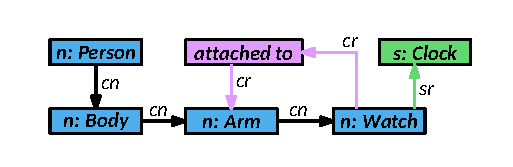
\includegraphics[width=0.7\textwidth]{chapter/chapter_2/mmfg-ex.eps}
    \caption{Beispiel für den Multimedia Feature Graphen $MMFG_{ex}$.}
    \label{sec2:sota:subsec:fz-explainablity:fig:mmfg-example}
\end{figure}

\paragraph{Erklärbarkeit von MMFGs}
\label{sec2:sota:par:explainability-of-mmfgs}
Um Erklärbarkeit von MMFGs zu erreichen, muss die technische Darstellung der Merkmale in eine für Menschen verständliche Bedeutung überführt werden.
Das Überbrücken dieser Lücke ist nicht in einem einzigen Schritt machbar.
Es benötigt mehrere Schritte, um diese Lücke zu schließen.
In einem ersten Zwischenschritt muss die Lücke zwischen der technischen Darstellung der Merkmale und ihrer semantischen Darstellung überbrückt werden.
Hierzu wird ein formaler und für Maschinen lesbarer Ansatz zur Erweiterung von MMFGs benötigt \cite{towards_auto_sem_expl_mmfg}.
In verwandten Arbeiten, wie \cite{towards_auto_sem_expl_mmfg}, wurden umfangreiche Konzepte entwickelt und beschrieben, die in der Lage sind durch Erweiterungen von MMFGs Erklärbarkeit zu erreichen.
Das Überbrücken der Lücke zwischen der technischen Darstellung der Merkmale und ihrer semantischen Darstellung gelingt mit einer semantischen Erweiterung.
Eine semantische Erweiterung von MMFGs kann durch das Anbinden eines externen Informationssystems, wie z.B. dem Semantic Web \cite{sem-web}, erreicht werden.
Durch das Definieren und Anwenden einer formalen kontextfreien Phrasenstruktur-Grammatik \cite{hausser-ps-grammar} in Kombination mit einer semantischen Erweiterung sind die Darstellungen von MMFGs nicht nur für Menschen lesbar, sondern es können auch für Menschen verständliche, sowie lesbare und auf natürlicher Sprache basierende Ausdrücke generiert werden.
Diese Erweiterungen ermöglichen formale semantische Darstellungen und schaffen die Grundlage für auf natürlicher Sprache basierende Erklärungen.
Diese Erweiterungen von MMFGs zu formalen semantischen Darstellungen führen zu Semantischen Multimedia Feature Graphen (SMMFGs) \cite{towards_auto_sem_expl_mmfg}, sowie zu Erklärbaren Semantischen Multimedia Feature Graphen (ESMMFGs) \cite{towards_auto_sem_expl_mmfg}.

Jeder auf natürlicher Sprache basierende Ausdruck, der mit solch einer Grammatik generiert wird, ist inhaltlich \textit{korrekt}, da es nur die ursprünglichen identifizierten Merkmale in einer formalen und für Menschen lesbaren Form darstellt \cite{towards_auto_sem_expl_mmfg}.
Auf diese Weise kann jedes Element eines MMFG bzw. identifizierte Merkmal strukturell und semantisch dargestellt werden \cite{towards_auto_sem_expl_mmfg}.
Des Weiteren bieten sich anhand der Grammatik und ihrer Produktionsregeln unbegrenzte Möglichkeiten zur Konstruktion natürlicher Ausdrücke \cite{towards_auto_sem_expl_mmfg}.
Durch Anpassungen der Produktionsregeln können Applikationen individuell die Konstruktion natürlicher Ausdrücke bestimmen \cite{towards_auto_sem_expl_mmfg}.
Anhand dieser Techniken können bereits gute Ergebnisse bzw. Erklärungen erzielt werden.
Besonders textbasierte Dokumente können mit dieser Herangehensweise erklärt werden, da die Struktur des MMFGs der Struktur des Dokuments folgt \cite{towards_auto_sem_expl_mmfg}.
Dies gilt allerdings nicht für andere Multimedia-Dateien, wie z.B. Bildern.
Für diese Dateitypen bleibt die Reihenfolge der konstruierten Sätze zufällig \cite{towards_auto_sem_expl_mmfg}.

Wichtig anzumerken ist, dass diese Konzepte ohne maschinelles Lernen auskommen und einen rein mathematischen und statistischen Ansatz verfolgen, um Erklärungen anhand identifizierter Merkmale zu generieren \cite{towards_auto_sem_expl_mmfg}.

\paragraph{Verarbeitung von MMFGs}
\label{sec2:sota:par:processing-of-mmfgs}
Der steigende Detaillierungsgrad (LOD) vieler multimedialer Inhalte führt zu einem Anstieg in der Anzahl an Elementen in einem MMFG \cite{exp-mmfg}.
So können in der Praxis MMFGs tausende Knoten und Kanten enthalten \cite{ai-based-sem-ind-retr-soc}.
Ein höherer Detaillierungsgrad und eine höhere Anzahl an Elementen in einem MMFG stärkt zwar die Wirksamkeit der Ergebnisse von Berechnungen eines MMFGs, wie z.B der Berechnung der Ähnlichkeit zweier MMFGs, sorgt aber allgemein auch für eine komplexere Graphenstruktur \cite{fast-effec-retr-large-collec}.
Diese Eigenschaft von MMFGs birgt eine Reihe von Problemen.
Zum einen ist die Umsetzung aktueller Algorithmen, wie z.B. zur Bestimmung der Ähnlichkeit von MMFGs, auf rechenschwachen Systemen, wie z.B Smartphones, mit dieser Anzahl an Knoten und Kanten aufgrund Speicherplatz und Laufzeitbegrenzungen nicht einfach zu handhaben und zum anderen sind aktuelle Algorithmen, die auf dem Durchlaufen eines Graphen basieren, wie z.B die Bestimmung der Ähnlichkeit zweier MMFGs, bei solch einer Anzahl an Knoten und Kanten nicht mehr effizient und zudem sehr rechenaufwendig \cite{fast-effec-retr-large-collec}.

Mathematisch betrachtet können Graphen durch ihre Adjazenzmatrix dargestellt werden \cite{fast-effec-retr-large-collec}.
Basierend auf einer Adjazenzmatrix können weitere Umformungen und Berechnungen durchgeführt werden \cite{fast-effec-retr-large-collec}. Ein Beispiel hierfür ist die Umwandlung eines Graphen in einen n-dimensionalen Vektorraum. Auf diesem Vektorraum können dann wiederum weitere Berechnungen durchgeführt werden.
Speziell für gewichtete Graphen, zu welchen auch per Definition MMFGs zählen, werden in der Regel Matrizen angewandt \cite{fast-effec-retr-large-collec}.
Diese Matrizen erweitern eine Adjazenzmatrix um die Gewichtung der Kanten.
Im weiteren Verlauf dieser Arbeit werden diese Matrizen auch Wertungsmatrizen (engl. valuation matrices) genannt.
Basierend auf diesen Darstellungen können mathematische Konzepte angewandt werden.
Ein Beispiel für so ein mathematisches Konzept ist die Anwendung der Eigenwert-Methode, durch welche eine auf Merkmale bezogene Ähnlichkeitsberechnung von Adjanzenzmatrizen durchgeführt werden kann \cite{fast-effec-retr-large-collec}.
Die Eigenwert-Methode reduziert eine quadratische Matrix $M$ auf eine einfache rationale Zahl $\lambda$ unter der Annahme $\exists~\Vec{v}: M \cdot \Vec{v} = \lambda \cdot \Vec{v}$ \cite{fast-effec-retr-large-collec}.
Auf diese Weise können Ähnlichkeitsberechnungen auf $\lambda$ anstatt der gesamten Matrix $M$ durchgeführt werden \cite{fast-effec-retr-large-collec}.
Allerdings weisen viele dieser Algorithmen eine polynomielle Laufzeit von $\mathcal{O}((n + e)^2)$ oder gar exponentielle Laufzeit auf (hierbei verweist $n$ auf die Anzahl der Knoten und $e$ auf die Anzahl der Kanten) \cite{fast-effec-retr-large-collec}.
Um effektive und effiziente Verarbeitungen, wie z.B. Abfragen, für große Datenstrukturen und Sammlungen multimedialer Inhalte, wie einem MMFG, zu ermöglichen, müssen effizientere Algorithmen, wie zur Bestimmung der Ähnlichkeit von MMFGs, die mit komplexeren Graphenstrukturen umgehen können, eingesetzt werden \cite{fast-effec-retr-large-collec}.

Im nächsten Abschnitt wird eine Projektion eines Graphen in einen zweidimensionalen Vektorraum, sowie entsprechende Algorithmen vorgestellt.
Diese Projektion stellt eine Erweiterung der Wertungsmatrix eines Graphen dar und ermöglicht statt einer exponentiellen Komplexität der Laufzeit eine lineare Laufzeitkomplexität von $\mathcal{O}(n+e)$ und unterstützt zudem ein höheren Detaillierungsgrad von MMFGs \cite{fast-effec-retr-large-collec}.
Das Konzept dieser Projektion wird im weiteren Verlauf der Arbeit als Graph Code \cite{gc-2d-proj-mmfg} bezeichnet.


\subsubsection{Graph Codes}
\label{sec2:sota:subsubsec:graph-codes}
In diesem Abschnitt werden die mathematischen und algorithmischen Konzepte der Graph Codes beschrieben.
Zuerst werden die Grundlagen von Graph Codes beschrieben.
Diese Grundlagen umfassen des Weiteren die in \cref{sec2:sota:par:gc-encoding} beschriebene Codierung von Graph Codes, sowie die in \cref{sec2:sota:par:gc-vocabulary-dictionary} beschriebenen technischen Eigenschaften, wie Vokabular und Wörterbücher von Graph Codes.
In \cref{sec2:sota:par:gc-similiarity} wird dann die Ähnlichkeit von Graph Codes behandelt.

Graph Codes sind eine Projektion eines MMFG in einen zweidimensionalen Raum \cite{gc-2d-proj-mmfg}.
Dabei basieren Graph Codes auf Operationen auf der Adjazenzmatrix eines Graphen und können allgemein, per Prinzip, auf jede Art von Graphen angewendet werden.
Allerdings wurden Graph Codes spezifisch für MMIR entwickelt.
Graph Codes werden eingesetzt, um MMFGs zu transformieren und in einer Form darzustellen, die schnelleres und effizienteres MMIR ermöglicht \cite{fast-effec-retr-large-collec}.
Grundlage dieser Umformung ist ein Algorithmus zur Codierung eines MMFG.
Dieser Algorithmus nimmt die Wertungsmatrix $WM$ eines MMFGs als Eingabe \cite{gc-2d-proj-mmfg}.
Um die grundlegenden Konzepte von Graph Codes vorzustellen, wird das Beispiel $MMFG_{ex}$ aus \cref{sec2:sota:subsec:fz-explainablity:fig:mmfg-example} als Basis benutzt.
Eine Wertungsmatrix enthält jeweils eine Zeile und Spalte für einen Knoten in einem MMFG.
Aufgrund dessen ist eine Wertungsmatrix auch eine quadratische Matrix.
Eine gerichtete Kante zwischen zwei Knoten $n_1$ und $n_2$ wird in der Wertungsmatrix durch ihre Gewichtung oder durch den Wert 1 im Eintrag $(n_1,n_2)$ der Wertungsmatrix $WM$ dargestellt.

Die Knoten \textit{Person, Body, Arm, Watch, Clock, attached to} des Beispiels $MMFG_{ex}$ werden in der Diagonalen der Wertungsmatrix ebenfalls durch den Wert 1 dargestellt.
Dies führt zu der in \cref{sec2:sota:subsec:fz-explainablity:fig:mmfg-valuation-matrix} dargestellten Wertungsmatrix.

%\begin{figure}[htb]
    \centering
    \resizebox{0.8\textwidth}{!}{
        \begin{tikzpicture}
            \node (tabl) {
                \begin{tabular}{rcccccc}
                     &  \begin{turn}{90}Person\end{turn}& \begin{turn}{90}Body\end{turn} & \begin{turn}{90}Arm\end{turn} & \begin{turn}{90}Watch\end{turn} & \begin{turn}{90}Clock\end{turn} & \begin{turn}{90}attached to $~$\end{turn} \\ \hline
                    Person      & 1 & 1 & 0 & 0 & 0 & 0 \\ 
                    Body        & 0 & 1 & 1 & 0 & 0 & 0 \\
                    Arm         & 0 & 0 & 1 & 1 & 0 & 0 \\ 
                    Watch       & 0 & 0 & 0 & 1 & 1 & 1 \\ 
                    Clock       & 0 & 0 & 0 & 0 & 1 & 0 \\ 
                    attached to & 0 & 0 & 1 & 0 & 0 & 1
                \end{tabular}
            };

            \node[anchor=south west] (wm) at([xshift=5mm]tabl.south east) {
                \shortstack[c]{
                    $WM(MMFG_{ex}) = $\\
                    \vspace*{1.5mm} \\
                    $\begin{pmatrix}
                    1 & 1 & 0 & 0 & 0 & 0  \\
                    0 & 1 & 1 & 0 & 0 & 0  \\
                    0 & 0 & 1 & 1 & 0 & 0  \\
                    0 & 0 & 0 & 1 & 1 & 1  \\
                    0 & 0 & 0 & 0 & 1 & 0  \\
                    0 & 0 & 1 & 0 & 0 & 1  \\
                    \end{pmatrix}$
                }
            };

            %\node[draw, fit=(tabl)(wm)] {};
        \end{tikzpicture}
    }
    \caption{Wertungsmatrix des Beispiels $MMFG_{ex}$.}
    \label{sec2:sota:subsec:fz-explainablity:fig:mmfg-valuation-matrix}
\end{figure}
\begin{figure}[htb]
    \centering
    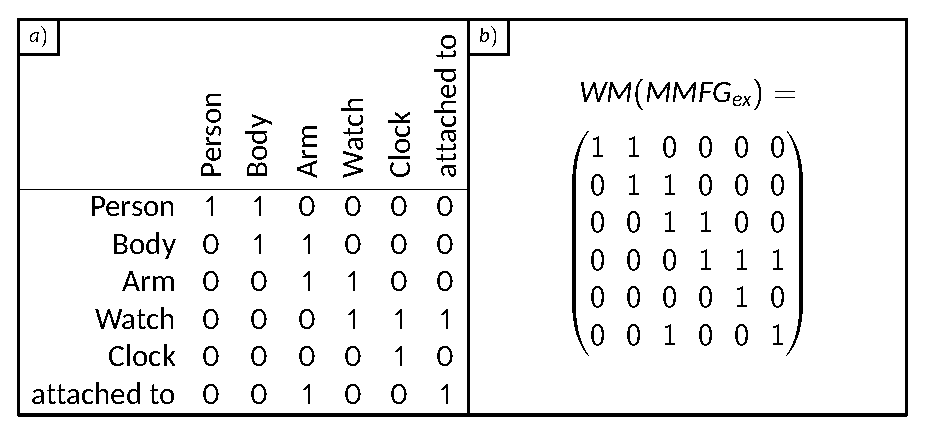
\includegraphics[width=\textwidth]{chapter/chapter_2/valuation-matrix-a-b.eps}
    \caption{Wertungsmatrix des Beispiels $MMFG_{ex}$ in a) Tabellenform und b) Form einer Matrix.}
    \label{sec2:sota:subsec:fz-explainablity:fig:mmfg-valuation-matrix}
\end{figure}

\paragraph{Codierung von Graph Codes}
\label{sec2:sota:par:gc-encoding}
Graph Codes wenden eine Funktion $f_{enc}$ zur Codierung von Informationen in einem MMFG an.
Diese Funktion codiert die Informationen zu den Typen der Knoten oder Kanten und ihren entsprechenden Attributen.
Hierzu werden für alle Einträge bzw. Felder in der Wertungsmatrix $WM$, die nicht null sind, numerische Werte berechnet.
Die Funktion $f_{enc}$ zur Codierung dieser Informationen kann von Applikationen je nach ihren jeweiligen Anforderungen angepasst werden \cite{gc-2d-proj-mmfg}.
Eine beispielhafte Codierung kann wie folgt lauten: Knoten = 1, Blatt = 2, Kindbeziehung = 3, Synonymbeziehung = 4, Beziehung = 5, Knoten (räumliche Beziehung) = 6, Knoten (Synonym) = 7.
Angewandt auf das Beispiel $MMFG_{ex}$ führt diese Codierung zu folgender in \cref{sec2:sota:subsec:fz-explainablity:fig:mmfg-valuation-matrix-enc} a-b) dargestellten codierten Wertungsmatrix $WM_{enc}$ bzw. Graph Code $GC_{ex}$.
Die Farben der Einträge in \cref{sec2:sota:subsec:fz-explainablity:fig:mmfg-valuation-matrix-enc} entsprechen der Färbung der Knoten aus \cref{sec2:sota:subsec:fz-explainablity:fig:mmfg-example}.
Die dazugehörigen Beziehungen sind ebenfalls entsprechend gefärbt.
\cref{sec2:sota:subsec:fz-explainablity:fig:mmfg-valuation-matrix-enc} c) hingegen zeigt den durch das GMAF generierten Graph Code $GC_{ex}$ des Beispiels $MMFG_{ex}$.
Es sei angemerkt, dass die Unterschiede zwischen dem Graph Code $GC_{ex}$ aus \cref{sec2:sota:subsec:fz-explainablity:fig:mmfg-valuation-matrix-enc} a-b) und \cref{sec2:sota:subsec:fz-explainablity:fig:mmfg-valuation-matrix-enc} c) durch die vom GMAF eigens definierte Funktion $f_{enc}$ zustande kommen.
Des Weiteren inkludiert das GMAF die Synonym-Knoten $Clock$ und $attached~to$ nicht in seiner Abbildung.
Die Beziehung $attached~to$ wird im GMAF durch den Eintrag $(Arm,Watch)$ im Graph Code $GC_{ex}$ dargestellt.
Hier wird eine feinere Differenzierung der räumlichen Beziehung vorgenommen und durch den Wert 17 dargestellt.
Durch komplexere Funktionen zur Codierung können Attribute, Gewichtung oder auch andere Informationen in einem MMFG codiert und durch beliebige Zahlen dargestellt werden, welche im weiteren Verlauf einer Verarbeitung gezielt genutzt werden können.

\begin{figure}[htb]
    \centering
    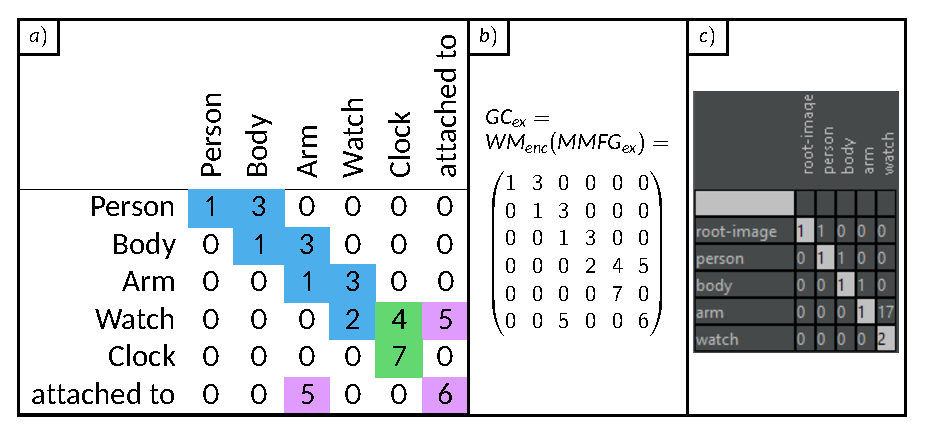
\includegraphics[width=\textwidth, keepaspectratio]{chapter/chapter_2/valuation-matrix-enc.eps}
    \caption{Codierte Wertungsmatrix bzw. Graph Code $GC_{ex}$ zum entsprechenden Beispiel $MMFG_{ex}$in a) Tabellenform und b) in Form einer Matrix. c) Vom GMAF generierte Graph Code $GC_{ex}$.}
    \label{sec2:sota:subsec:fz-explainablity:fig:mmfg-valuation-matrix-enc}
\end{figure}

%\begin{figure}[htb]
    \centering
    \resizebox{0.8\textwidth}{!}{
        \begin{tikzpicture}

            \definecolor{nodeblue}{RGB}{76, 174, 234}
            \definecolor{syngreen}{RGB}{100, 216, 112}
            \definecolor{comprel}{RGB}{224, 155, 254}
            
            \node (tabl) {
                \begin{tabular}{rcccccc}
                     &  \begin{turn}{90}Person\end{turn}& \begin{turn}{90}Body\end{turn} & \begin{turn}{90}Arm\end{turn} & \begin{turn}{90}Watch\end{turn} & \begin{turn}{90}Clock\end{turn} & \begin{turn}{90}attached to $~$\end{turn} \\ \hline
                    Person      & \cellcolor{nodeblue}1 & \cellcolor{nodeblue}3 & 0 & 0 & 0 & 0 \\ 
                    Body        & 0 & \cellcolor{nodeblue}1 & \cellcolor{nodeblue}3 & 0 & 0 & 0 \\
                    Arm         & 0 & 0 & \cellcolor{nodeblue}1 & \cellcolor{nodeblue}3 & 0 & 0 \\ 
                    Watch       & 0 & 0 & 0 & \cellcolor{nodeblue}2 & \cellcolor{syngreen}4 & \cellcolor{comprel}5 \\ 
                    Clock       & 0 & 0 & 0 & 0 & \cellcolor{syngreen}7 & 0 \\ 
                    attached to & 0 & 0 & \cellcolor{comprel}5 & 0 & 0 & \cellcolor{comprel}6
                \end{tabular}
            };

            \node[anchor=south west, right=1cm of tabl.east] (wm) {
                \shortstack[l]{
                    $GC_{ex} = $ \\
                    $WM_{enc}(MMFG_{ex}) = $\\
                    \vspace*{1.5mm} \\
                    $\begin{pmatrix}
                    1 & 3 & 0 & 0 & 0 & 0  \\
                    0 & 1 & 3 & 0 & 0 & 0  \\
                    0 & 0 & 1 & 3 & 0 & 0  \\
                    0 & 0 & 0 & 2 & 4 & 5  \\
                    0 & 0 & 0 & 0 & 7 & 0  \\
                    0 & 0 & 5 & 0 & 0 & 6  \\
                    \end{pmatrix}$
                }
            };
        \end{tikzpicture}
    }
    \caption{Codierte Wertungsmatrix bzw. Graph Code $GC_{ex}$ zum entsprechenden Beispiel $MMFG_{ex}$.}
    \label{sec2:sota:subsec:fz-explainablity:fig:mmfg-valuation-matrix-enc}
\end{figure}

%\begin{figure}[htb]
%    \centering
%    \includegraphics{chapter/chapter_2/gc-ex1.png}
%    \caption{Vom GMAF generierter Graph Code $GC_{ex}$ des Beispiels $MMFG_{ex}$.}
%    \label{sec2:sota:subsec:fz-explainablity:fig:gmaf-gc-ex1}
%\end{figure}

Bei der Berechnung der Ähnlichkeit von Graph Codes müssen diese miteinander verglichen werden.
Damit Graph Codes verglichen werden können, muss der Vergleich dieser Graph Codes auf einer genaustens definierten Metrik für Ähnlichkeit beruhen.
Diese Metrik muss die mathematischen Aspekte eines Vergleichs von Matrizen und auch die semantischen Aspekte von Graph Codes berücksichtigen \cite{gc-2d-proj-mmfg}.
Im nächsten \cref{sec2:sota:par:gc-vocabulary-dictionary} werden weitere grundlegende Definitionen eingeführt und definiert, die zur Definition einer Metrik zur Ähnlichkeit von Graph Codes notwendig sind und eine Berechnung der Ähnlichkeit von Graph Codes unabhängig von den Typen der Knoten und Kanten ermöglicht.

\paragraph{Vokabular und Wörterbuch eines Graph Codes}
\label{sec2:sota:par:gc-vocabulary-dictionary}
Die Menge der Knoten $V$ in einem MMFG, welche die identifizierten Merkmale darstellen, können als eindeutige Bezeichner für das Vokabular bzw. die Gesamtheit aller Wörter, welche einen MMFG ausmachen, betrachtet werden.
Die Menge dieser Bezeichner wird mit $FVT_{MMFG}=\{fvt_1,...,fvt_n\}$ notiert und stellt somit die Elemente des \enquote{Wörterbuchs} eines Graph Codes dar.
Damit ein Bezeichner $fvt_i$ eines Eintrages in einem Graph Code eindeutig identifiziert werden kann, wird ein Vektor $dict_{GC}$ definiert.
Dieser Vektor bietet eine geordnete Reihenfolge für die Menge an Bezeichner $FVT_{MMFG}$ und weist jedem Bezeichner eine eindeutig definierte Position zu.
Die Ordnung dieser Bezeichner im Vektor $dict_{GC}$ kann durch eine beliebige Strategie, wie z.B. durch Breitensuche, Tiefensuche oder manuell, erfolgen.
Durch den Vektor $dict_{GC}$ kann jedes Feld in der Diagonalen des entsprechenden Graph Codes einem Eintrag im Wörterbuch, dargestellt durch $dict_{GC} = (fvt_1,...,fvt_n)$, zugeordnet werden \cite{gc-2d-proj-mmfg}.
Angewandt auf den Graph Code $GC_{ex}$ ergibt sich für die Menge an Bezeichnern $FVT_{ex}=\{Person,Body,Arm,Watch,Clock,attached~to\}$, sowie der Vektor $dict_{ex}=(Person,Body,Arm,Watch,Clock,attached~to)$.
Die Reihenfolge der Bezeichner in $FVT_{ex}$ ist unerheblich und ist für gewöhnlich zufällig.

Anders als $FVT_{ex}$ weist $dict_{ex}$ eine spezifische Reihenfolge auf, die in \cref{sec2:sota:par:gc-vocabulary-dictionary:tab:dict-ex} dargestellt wird.

\begin{table}[htb]
    \centering
    \begin{tabular}{c|c|c|c|c|c|c}
         Index $i$ & 1 & 2 & 3 & 4 & 5 & 6 \\ \hline
         $fvt_i$ & Person & Body & Arm & Watch & Clock & attached to
    \end{tabular}
    \caption{$dict_{ex}$ vom Graph Code $GC_{ex}$.}
    \label{sec2:sota:par:gc-vocabulary-dictionary:tab:dict-ex}
\end{table}

Beim Vergleichen von Graph Codes ist es wichtig nur die Einträge äquivalenter Merkmale in den Diagonalen der Graph Codes miteinander zu vergleichen.
Da jeder Graph Code einen individuellen Vektor $dict_{GC}$ mit individueller Ordnung besitzt, unterscheiden sich die Wörterbücher der Graph Codes für gewöhnlich voneinander $dict_{GC_1} \neq dict_{GC_2}$.
Äquivalente Merkmale können durch die Schnittmenge der Bezeichner bestimmt werden: $FVT_{1 \cap 2} = \{fvt_1,...,fvt_n\} = V_{MMFG_1} \cap V_{MMFG_2}$.
Analog kann dieses Prinzip auch auf die Wörterbücher von Graph Codes angewendet werden: $dict_{1 \cap 2 } = dict_{GC_1} \cap dict_{GC_2}$.
Aufgrund der unterschiedlichen Ordnungen der Wörterbücher von Graph Codes können diese nicht einfach miteinander verglichen werden, da die Einträge in den zu vergleichenden Graph Codes unterschiedliche Bezeichner darstellen.
Um diesem Problem zu begegnen und die Ordnung von Graph Codes anzupassen, gibt es eine Äquivalenzfunktion $f_{equ}(M_{\cap})$, die die Matrix der Schnittmenge der Wertematrizen bzw. das Wörterbuch so transformiert, dass das entsprechende Wörterbuch nach dem Vektor bzw. Wörterbuch $dict_{\cup}$ geordnet ist \cite{gc-2d-proj-mmfg}.

Konträr zur Schnittmenge kann auch eine Vereinigung von Graph Codes erfolgen.
Eine Vereinigung kann dann erfolgen, wenn eine Applikation eine Sammlung an MMFGs enthält.
Im Falle der Vereinigung von Graph Codes werden die Menge der Bezeichner, sowie die Wörterbücher der Graph Codes miteinander vereint.
Die Gesamtheit aller Bezeichner $FVT_{Coll}$ kann als Vereinigung aller Bezeichner in der Sammlung an MMFGs definiert werden und als Vereinigung aller Wörterbücher dargestellt werden $dict_{\cup}: FVT_{Coll} = \bigcup^{n}_{i=1} FVT_{MMFG_i}$ mit $\forall i,j < n: dict_{\cup} = dict_i \times dict_j$.
Um die Vereinigung der Wörterbücher zu erstellen, wird jedes Wörterbuch $dict_i$ durchlaufen und, sofern noch nicht im Wörterbuch $dict_{\cup}$ vorhanden, jeder individueller Bezeichner hinzugefügt.
Wird ein $dict_{\cup}$ aus der vollständigen Sammlung an Graph Codes berechnet, so kann $dict_{\cup}$ als ein globales Wörterbuch betrachtet werden, in welchem jeder einzigartige Bezeichner eine einzigartige Position besitzt \cite{gc-2d-proj-mmfg}.

%Im folgenden Abschnitt wird anhand der in diesem Abschnitt eingeführten Definitionen eine Metrik zur Ähnlichkeit von Graph Codes vorgestellt und beschrieben.

% Die in diesem Abschnitt beschriebenen Definitionen ermöglichen eine effiziente und effektive Verarbeitung von Informationen von Graph Codes...
% Im nächsten Abschnitt wird solch eine Verarbeitung, die Berechnung der Ähnlichkeit zweier Graph Codes beschrieben.
% Die Berechnung ist ein gutes Beispiel, da es in unterschiedlichsten Anwendungsfällen, wie der Bestimmung der Gemeinsamkeiten oder Unterschiede Verwendung finden kann.

Die in diesem Abschnitt beschriebenen Definitionen ermöglichen eine effiziente und effektive Verarbeitung von Informationen eines Graph Codes.
Ein Beispiel für so eine Verarbeitung ist die Berechnung der Ähnlichkeit zweier Graph Codes, die auf einem Vergleich dieser beiden basiert.
Wie bereits erwähnt, muss der Vergleich dieser Graph Codes auf einer genaustens definierten Metrik beruhen.
%Mit Hilfe dieser Metriken können Eigenschaften von Graph Codes quantifiziert werden und
Im nächsten Abschnitt werden diese Metriken vorgestellt.

\paragraph{Ähnlichkeit von Graph Codes}
\label{sec2:sota:par:gc-similiarity}
In diesem Abschnitt wird eine Metrik zur Berechnung der Ähnlichkeit bzw. zum Vergleich von Graph Codes beschrieben.
Die in diesem Abschnitt vorgestellten Metriken wurden aus \cite{gc-2d-proj-mmfg} entnommen und ermöglichen die Quantifizierung der Eigenschaften von Graph Codes.
Diese Metrik muss die Zeilen, Spalten und die Einträge, die die Knoten und Kanten darstellen, berücksichtigen.
D.h. diese Metrik zur Berechnung der Ähnlichkeit von Graph Codes muss auf Matrizen anwendbar sein, dessen Zeilen und Spalten die Knoten und Kanten eines MMFGs darstellen.
Damit ein Vergleich dieser Einträge möglich ist, müssen die Einträge vom selben Typ sein.
Da die Wörterbücher von Graph Codes für gewöhnlich unterschiedlich sind, ist es zudem wichtig die korrekten Einträge in einer Matrix zu vergleichen \cite{gc-2d-proj-mmfg}.
Es kann zwischen drei Typen an Einträgen differenziert werden:
\begin{itemize}
    \item Knoten (stellt Merkmale dar)
    \item Kanten (Beziehungen zwischen Knoten bzw. Merkmalen)
    \item Kantentyp (Typ der Beziehung zwischen Knoten bzw. Merkmalen)
\end{itemize}
Für jeden Typ eines Eintrages kann jeweils eine eigene Metrik definiert werden:
\begin{itemize}
    \item Metrik für Merkmale $M_F$
    \item Metrik für Merkmalsbeziehungen $M_{FR}$
    \item Metrik für Beziehungstypen $M_{RT}$
\end{itemize}
Diese Metriken können wiederum als Tripel in einer Metrik $M_{GC} = (M_F, M_{FR}, M_{RT})$ zusammengefasst werden und bilden die gesamte Metrik, die die Ähnlichkeit von Graph Codes darstellen soll.
Diese Metriken werden im Folgenden vorgestellt und beschrieben.

% Metriken eindampfen
% Was ist die Aufgabe einer Metrik?
% Was zeichnet diese Metrik aus?
% Anwendungsbeispiel bzw. fall einer Metrik?
% Nochmal über den technischen Aspekt nachdenken...

Die \textbf{Metrik für Merkmale} $M_F$ berechnet die Ähnlichkeit von Graph Codes anhand der Schnittmenge der Bezeichner in einem Wörterbuch.
Die Metrik $M_F$ ist definiert als das Verhältnis zwischen der Kardinalität der Schnittmenge von Bezeichnern $dict_{\cap}$ der Wörterbücher $dict_i$ und $dict_j$ der Graph Codes $GC_i$ und $GC_j$ und der Kardinalität des Wörterbuchs $dict_i$ vom Graph Code $GC_i$.
Die Formel für diese Metrik lautet $M_F(GC_i, GC_j) = \frac{\abs{dict_{\cap}}}{\abs{dict_i}}$.
Hierbei bezeichnet $\abs{\Vec{v}}$ die Kardinalität eines Vektors, sprich die Anzahl der Elemente in einem Vektor.
Anders formuliert, ist der Wert der Ähnlichkeit höher, desto mehr Merkmale zwei Graph Codes gemeinsam haben.
Es ist wichtig anzumerken, dass diese Metrik nur Knoten bzw. Merkmale betrachtet, unabhängig von den Beziehungen zwischen diesen Merkmalen \cite{gc-2d-proj-mmfg}.

Die \textbf{Metrik für Merkmalsbeziehungen} $M_{FR}$ ist die Grudlage für die Berechnung der Ähnlichkeit von Beziehungen zwischen Merkmalen.
Beziehungen in einem Graph Code werden durch Einträge dargestellt, die nicht in der Diagonalen der Matrix vorkommen und deren Wert größer null ist.
Dabei bezieht die Berechnung dieser Metrik nur Einträge aus der Schnittmenge $M_{\cap}$ der Matrizen ein, die Beziehungen mit demselben Ausgang- und Zielknoten darstellen.
Die Berechnung dieser Metrik basiert auf den nicht in der Diagonalen vorkommenden Einträgen der Adjazenzmatrix $AM(M_{\cap})$.
Die Metrik $M_{FR}$ ist definiert als das Verhältnis zwischen der Summe aller nicht in der Diagonalen vorkommenden Einträge und der Kardinalität aller nicht in der Diagonalen vorkommenden Einträge.
Die Formel für diese Metrik lautet $M_{FR}(GC_i, GC_j) = \frac{\Sigma AM(M_{i~\cap~j}) -n}{\abs{AM(M_{\cap~i})} - n}$.
Die Metrik $M_{FR}$ stellt somit das Verhältnis zwischen der Zahl der Einträge, die Beziehungen darstellen und der Anzahl der äquivalenten und in der Schnittmenge vorkommenden Einträge, die Beziehungen darstellen, von Graph Codes.
Somit zählt die Metrik $M_{FR}$ die Anzahl aller Beziehungen zwischen Ausgangs- und Zielknoten.
Die Metrik berücksichtigt jedoch nicht die Äquivalenz der Typen der Beziehungen.
Die Äquivalenz der Typen von Beziehungen wird von der nächsten Metrik, der Metrik für Beziehungstypen berücksichtigt \cite{gc-2d-proj-mmfg}.

Die \textbf{Metrik für Beziehungstypen} $M_{RT}$ basiert auf der Metrik für Merkmalsbeziehungen.
Die Codierungsfunktion $f_{enc}$ codiert für verschiedene Typen von Beziehungen unterschiedliche Werte.
Eine Ähnlichkeit von Typen von Beziehungen setzt aber voraus, dass die Einträge, die die Beziehungen darstellen, vom selben Typ sind, damit sie verglichen werden können.
Diese Metrik führt die Berechnungen nicht mehr anhand der Adjazenzmatrix der zu vergleichenden Graph Codes aus, sondern anhand der Schnittmenge $M_{\cap}$ der codierten Wertungsmatrizen.
Bei dieser Berechnung wird die Subtraktion auf äquivalenten Einträgen der zu vergleichenden Graph Codes durchgeführt.
Ist das Ergebnis dieser Subtraktion gleich null, so ist der Typ der Beziehung äquivalent.
Sind alle äquivalenten Einträge gleich, so ist die Summe der Subtraktionen dieser Einträge zueinander gleich null.
Im Vergleich zur Metrik $M_{FR}$, die nur Berechnungen anhand einer Adjazenzmatrix durchführt, verwendet diese Metrik zusätzlich den Wert der Codierung, welche den Typ der Beziehung darstellt, um festzustellen, ob die verglichenen Typen äquivalent sind.
Die Metrik $M_{RT}$ ist definiert als das Verhältnis zwischen der Summe aller nicht in der Diagonalen vorkommenden Einträge und der Kardinalität dieser Einträge.
Die Formel für diese Metrik lautet $M_{RT}(GC_i,GC_j) = \frac{\Sigma^{n,i \neq j}_{i,j}(\abs{M_{\cap i} - M_{\cap j}})}{\abs{M_{\cap i} - n}}$ \cite{gc-2d-proj-mmfg}.

\paragraph{Erklärbarkeit von Graph Codes}
Analog zur Erklärbarkeit von MMFGs in \cref{sec2:sota:par:explainability-of-mmfgs}, muss die technische Darstellung der Merkmale in eine für Menschen verständliche Bedeutung überführt werden.
Auch hier gilt es in einem ersten Schritt die Lücke zwischen der technischen Darstellung und ihrer semantischen Darstellung zu überbrücken.
Die semantische Darstellung von Merkmalen wurde in \cref{sec2:sota:par:explainability-of-mmfgs} bereits durch das Anbinden von externen Informationssystemen erreicht und resultierte in SMMFGs.
Das Anwenden der Algorithmen von Graph Codes auf SMMFGs ermöglicht die semantische Darstellung von Merkmalen in Graph Codes und führt zu Sementischen Graph Codes (SGCs) \cite{towards_auto_sem_expl_mmfg}.
Während das Wörterbuch eines Graph Codes die Menge der Bezeichner der Merkmale darstellt, stellt das Wörterbuch eines Semantischen Graph Codes die semantische Darstellung der Bedeutung dieser Bezeichner dar.
Analog zu MMFGs können auch für Graph Codes, durch das Definieren und Anwenden einer formalen kontextfreien Phrasenstruktur-Grammatik in Kombination mit Semantischen Graph Codes, für Menschen lesbare, verständliche und auf natürlicher Sprache basierende Ausdrücke generiert werden.
Die Erweiterung von Graph Codes um eine formale kontextfreie Grammatik führt zu Erklärbaren Semantischen Graph Codes (ESGCs) \cite{exp-mmfg}.

In Bezug auf Graph Codes ist wichtig anzumerken, dass Graph Codes nicht einen allgemeinen Ersatz bzw. eine allgemeine Alternative zu MMFGs darstellen und nur in bestimmten Fällen, wie z.B. beim Vergleich von MMFGs zur Bestimmung der Ähnlichkeit, eine Verbesserung bieten \cite{gc-2d-proj-mmfg}.
Des Weiteren werden Erklärungen von Graph Codes bislang nur anhand statistischer und rein mathematischer Vorgehensweisen erzeugt.
Es existiert keine Möglichkeit oder Untersuchung Systeme generativer KI zur Erklärbarkeit von Graph Codes zu nutzen.
Dies führt zur ersten offenen Herausforderung.

\begin{tcolorbox}[minipage, colback=white, colframe=black, arc=0pt, outer arc=0pt]
    \textbf{Offene Herausforderung OH 1.1 - Erklärbarkeit durch generative KI} \\
    Einsatz von generativer KI als Ersatz bzw. Alternative zur statistischen und rein mathematischen Vorgehensweise, um Erklärungen zu generieren.
    % Einsatz von generativer KI als Ersatz zur statistischen und rein mathematischen Vorgehensweise, um Erklärungen für Graph Codes zu generieren.
\end{tcolorbox}

Die offene Herausforderung \openissue{sec2:sota:oi:1.1}{OH 1.1} hat in Bezug auf dieses Forschungsziel einen konkretisierenden Charakter.
Das Forschungsziel bezieht sich in erster Linie auf Erklärbarkeit von MMIR im Allgemeinen und untersucht hierfür bereits bestehende Verfahren, mit welchen Erklärungen zu Datenstrukturen, wie den MMFGs oder Graph Codes, erzeugt werden können.
Die offene Herausforderung bezieht sich hingegen direkt auf die Datenstruktur der Graph Codes und verdeutlicht, dass es keine Möglichkeit gibt, mittels generativer KI Erklärungen für Graph Codes zu erzeugen.

Die offene Herausforderung \textbf{OH 1.1} wird im Rahmen einer Modellierung, sowie Implementierung in jeweils \hyperref[sec3:model:subsec:fz-explainability]{FZ 1.2/TB} und \hyperref[sec4:impl:subsec:fz-explainability]{FZ 1.3/I} angesprochen und untersucht.

\subsubsection{Generative KI}
\label{sec2:sota:subsubsec:genai}
Generative künstliche Intelligenz (GenKI, engl. generative AI (GenAI)) ist ein Typ künstlicher Intelligenz, die es ermöglicht, anhand vorhandener Informationen und Vorgaben, eine große Vielfalt an neuen Inhalten zu erstellen.
Beispiele für diese Inhalte können Bilder, Videos, Audiodateien, Texte oder anderweitige synthetische Daten sein \cite{gen-ai-tech-target}.
Synthetische Daten bezeichnet Daten, die nicht auf natürliche, sondern auf künstliche Art und Weise durch eine KI erstellt wurden, um echte Daten zu erweitern, oder zu ersetzen \cite{synt-data-ibm}.
Damit eine generative KI synthetische Daten erzeugen kann, wird das Modell der KI mithilfe eines Algorithmus anhand echter Daten so trainiert, dass es in der Lage ist, die ursprüngliche Struktur und die Eigenschaften, wie Muster, Zusammenhänge und statistische Merkmale, der echten Daten zu reproduzieren \cite{synth-data-eu, synth-mostlyai}.
Generative KI wird daher als generativ bezeichnet, da sie auf Grundlage bereits vorhandener Datensätze etwas Neues bzw. etwas bisher nicht Dagewesenes erzeugt.
Diese Eigenschaft hebt generative KI wesentlich von diskriminativer KI ab, welche einzig und allein zwischen verschiedenen Eingaben differenzieren kann \cite{computer-woche-genai}.

Ein Anwendungsbeispiel für eine diskriminative KI wäre eine simple binäre Klassifikation von Bildern und ob ein Bild eine Katze darstellt bzw. enthält, oder nicht.
Mit genügend Daten kann das diskriminative Modell einer KI so trainiert werden, dass es bestimmte Eigenschaften, wie Formen und Texturen, die einer Katze gleichen, in einem Bild erkennen kann.
Anhand erkannter Merkmale kann das Modell eine Vorhersage treffen, ob in einem Bild eine Katze zu sehen ist, oder nicht.
Eine wichtige Voraussetzung für das Training dieses Modells ist es, dass jede Beobachtung in den Trainingsdaten manuell mit einer Bezeichnung versehen ist.
Im Fall einer binären Klassifikation sind die Bilder, die Katzen darstellen bzw. enthalten, mit der Bezeichnung 1 versehen, alle anderen Bilder mit der Bezeichnung 0.
Durch das Training erlernt das diskriminative Modell beide Gruppen zu unterscheiden.

Die diskriminative Modellierung ist daher gleichbedeutend mit dem überwachten maschinellen Lernen (engl. supervised machine learning) \cite{orlly-deep-gen-learning}.
In der Tat wird ein Großteil der diskriminativen Modelle für überwachtes maschinelles Lernen verwendet \cite{turing-genai}.
Diskriminative KI bildet also die Eingabe eines mit Bezeichnungen versehenen Datensatzes auf eine Ausgabe ab.
Im Vergleich dazu benötigt das Training eines generativen Modells für gewöhnlich keine explizit mit Bezeichnungen versehenen Datensätze und kann somit mit dem nicht überwachten maschinellen Lernen (engl. unsupervised machine learning) gleichgesetzt werden.
Das Training auf einem mit Bezeichnungen versehenen Datensatz ist damit allerdings nicht ausgeschlossen und kann auch Verwendung finden \cite{orlly-deep-gen-learning}.

Es ist wichtig anzumerken, dass generative KI, die auf der Methode des Deep Learnings aufbaut, nicht neu ist und bereits in den 60ern in Form von Chatbots vorgestellt wurde \cite{gen-ai-tech-target}.
Die erste Instanz eines solchen Chatbots hieß \enquote{ELIZA} \cite{eliza} und wurde 1966 am MIT entwickelt und hatte zur Aufgabe Gespräche mit einem Psychotherapeuten zu simulieren \cite{computer-woche-genai}.
Durch das Aufkommen von künstlichen neuronalen Netzwerken (engl. articial neural networks (ANN)) und entsprechender Algorithmen in den 80ern und 90ern, sowie durch bessere Datenlage und Rechenkapazitäten wurde die Methode des Deep Learning praxistauglicher.
Die in 2014 von Ian Goodfellow vorgestellte Technik der generativen gegnerischen Netzwerke (engl. generative adversarial networks (GAN)) führte zu einem Durchbruch und ermöglichte es generativer KI überzeugend wirkende neuartige Inhalte zu generieren \cite{medium-genai-history}.

\paragraph{Grundlegende Techniken und Konzepte}
\label{sec2:sota:par:basic-concepts}
In diesem Abschnitt wird genauer auf wichtige Techniken und Technologien eingegangen, die in aktuellen generativen KI-Systemen Verwendung finden.
Die Techniken und Technologien werden kurz beschrieben und erläutert.
Zuerst werden die allgemeinen Techniken, wie Machine Learning oder Deep Learning vorgestellt bzw. rekapituliert und weiter wichtige Konzepte im Bereich der generativen KI angesprochen.
Die in diesem Abschnitt vorgestellten Techniken bzw. Technologien sind dabei so geordnet, dass sie einer logischen Abfolge in Bezug auf ihre Abhängigkeiten zueinander folgen.

\textbf{Machine Learning} (z.Dt. maschinelles Lernen) ist ein Teilbereich der KI \cite{machine-learning-big-data-insider} und hat zum Ziel die Art und Weise, wie Menschen lernen zu imitieren \cite{ai-ml-dl}.
Maschinelles Lernen ermöglicht es Systemen, Muster und Zusammenhänge automatisch und selbstständig aus Daten und Erfahrungen zu erlernen und zu verbessern, ohne dabei explizit programmiert zu sein \cite{machine-learning-data-absolut}.
Damit Machine Learning funktioniert und Muster und Zusammenhänge erlernt werden können, muss ein Datensatz zum Training vorhanden sein \cite{machine-learning-data-absolut}.
Im Bereich der KI spielen \textbf{(un)-supervised machine learning} (z.Dt. (un)-überwachtes maschinelles Lernen) eine zentrale Rolle \cite{machine-learning-big-data-insider}.
Überwachtes Lernen zeichnet sich dadurch aus, dass Algorithmen mithilfe von Daten trainiert werden, die im Trainingsdatensatz manuell mit Bezeichnungen versehen wurden \cite{machine-learning-data-absolut}.
Daher ist überwachtes Lernen mit einem relativ hohen menschlichen Aufwand verbunden \cite{machine-learning-data-absolut}.
Weit verbreitete Problemstellungen bzw. Aufgaben, in denen überwachtes Lernen eingesetzt werden, sind die Klassifikation und Regression \cite{machine-learning-algorithms-quick-review}.
Unüberwachtes Lernen zeichnet sich hingegen dadurch aus, dass es ohne die Einflussnahme von Menschen Gemeinsamkeiten, Unterschiede, Gruppen und Muster in Daten erkennen kann \cite{machine-learning-data-absolut}.
Unüberwachtes Lernen hat, aufgrund seiner Fähigkeit Muster eigenständig erlernen zu können, viele Anwendungsfälle und kann besonders für die Bildanalyse, wie Objekterkennung, oder für die Erkennung von Auffälligkeiten in Daten Verwendung finden \cite{machine-learning-ibm}.

\textbf{Deep Learning} (z.Dt. tiefes Lernen) ist eine besondere Form des maschinellen Lernens und ist in der Lage große Datenmengen zu verarbeiten \cite{deep-learning-ibm}.
Im Mittelpunkt des tiefen Lernens stehen \textbf{Articial Neural Networks (ANNs)} (z.Dt. künstliche neurale Netzwerke (KNN)), die ebenfalls ein Teilgebiet des maschinellen Lernens sind \cite{ibm-ai-ml-dl}.
Künstliche neuronale Netzwerke sind Algorithmen, deren Struktur und Verhalten nach dem biologischen Vorbild des menschlichen Gehirns und seiner Neuronen modelliert ist \cite{deep-learning-ibm,deep-learning-data-absolut}.
%Diese Netzwerke ermöglichen es Modellen tiefen Lernens komplexe Merkmale zu extrahieren und genaue Vorhersagen zu treffen.
Neuronale Netzwerke ermöglichen somit das Erlernen von komplexen Mustern und sind in der Lage genaue Vorhersagen zu treffen.
Da tiefes Lernen sehr rechenintensiv ist, kann es Monate dauern, bis Vorhersagen und Entscheidungen gute Ergebnisse liefern \cite{deep-learning-data-absolut}.
Ein sehr bekanntes Beispiel für ein neuronales Netzwerk ist der Suchalgorithmus von Google \cite{ibm-ai-ml-dl}.
Bekannte Modelle tiefen Lernens im Bereich der generativen KI sind \textbf{Generative Adverserial Networks (GANs)} \cite{goodfellow-gan} und \textbf{Variational Auto Encoders (VAEs)} \cite{kigma-vaes}.

%\textbf{Large Language Models (LLMs)} (z.Dt. großes Sprachmodell) sind große generative Sprachmodelle und stellen ein Teilbereich der KI dar.
%Die Architektur von LLMs basiert auf neuronalen Netzwerken, spezifischer \textbf{Transformern}.
%LLMs sind auf natürlicher Sprache trainiert und sind spezialisiert auf die Verarbeitung von natürlicher Sprache (NLP).
%D.h. LLMs sind in der Lage natürliche Sprache zu verstehen, zu verarbeiten und Ausdrücke natürlicher Sprache zu generieren.
%LLMs werden auf riesigen Textmengen trainiert und weisen in der Praxis Milliarden an Parameter auf.
%LLMs arbeiten mit Statistik und Wahrscheinlichkeitsverteilungen und optimieren mit diesen die Genauigkeit ihrer Vorhersage für die wahrscheinlichste Komplementierung des Textes \cite{towards-data-science-icl}.

\textbf{Large Language Models (LLMs)} (z.Dt. großes Sprachmodell) sind große generative Sprachmodelle und stellen einen Teilbereich der KI dar \cite{nvidia-llm}.
Eine sehr prominente Architektur von großen Sprachmodellen sind Transformer \cite{nvidia-llm}.
Die Architektur von Transformern basiert auf neuronalen Netzwerken und zeichnet sich dadurch aus, dass es Kontext und Bedeutung durch Beobachtung der Beziehungen zwischen Wörtern erlernen kann \cite{nvidia-llm}.
Transformer wurden zuerst von Google in \enquote{Attention Is All You Need.} \cite{google-attention} vorgestellt und führen zwei neue Techniken ein: positionelle Kodierung und Selbstaufmerksamkeit \cite{nvidia-llm}.
Große Sprachmodelle werden meist durch unüberwachtes Lernen auf riesigen Datenmengen trainiert und weisen in der Praxis Milliarden an Parameter auf \cite{nvidia-llm}.
Als solches erlernen LLMs die Muster der Statistiken und Wahrscheinlichkeitsverteilungen innerhalb der Trainingsdaten und optimieren mit diesen die Genauigkeit ihrer Vorhersagen anhand ihrer Anwendungsfälle \cite{towards-data-science-icl}.
Anwendungsfälle von Transformern sind vielfältig und können das z.B. Erzeugen, Übersetzen oder Zusammenfassen von Text umfassen \cite{nvidia-llm}.

\textbf{Explainable AI (xAI)} (z.Dt. erklärbare KI) befasst sich mit der Erklärbarkeit von KI.
Erklärbare KI beschäftigt sich u. a. mit der Frage \enquote{Wie kommt eine KI zu einem Ergebnis} und versucht die inneren Abläufe in einer KI zu beleuchten \cite{explainable-ai-kobold}.
Das generelle Problem mit KI ist, dass die Algorithmen wie neuronale Netzwerke und tiefes Lernen sogenannte \enquote{Black-Boxes} sind \cite{explainable-ai-kobold}.
Zwar ist die Funktionsweise dieser Algorithmen, sowie das finale Ergebnis bekannt, aber es ist nicht erkenntlich wie die KI dieses Ergebnis erreicht hat \cite{explainable-ai-kobold}.
Ziel von erklärbarer KI soll also sein, dass ein Mensch nachvollziehen kann, wie ein Algorithmus ein Ergebnis erreicht \cite{explainable-ai-kobold}.

Die meisten Systeme generativer KI arbeiten mit einer sogenannten \textbf{Prompt} (z.Dt. Eingabeaufforderung) als Eingabe.
Im Rahmen der Verarbeitung natürlicher Sprache und des maschinellen Lernens bezeichnet ein Prompt ein Stück Text, das als eine Anweisung an ein System verstanden werden kann und welches den Kontext und alle dazugehörigen und notwendigen Informationen enthält, damit ein Modell relevante Ausgaben erzeugen kann \cite{gradientpub-prompt,hopsworks-prompt-engineering}.
Anwendungsbeispiele für Prompts können Erklärungen, Fragen oder anderweitige Texteingaben sein.
Das Modell eines Systems verarbeitet die Eingabe und produziert in Abhängigkeit der Eingabe und der Fähigkeiten des jeweiligen Modells entsprechende Ausgaben, wie z.B. Vervollständigungen von Text, Erklärungen, Übersetzungen, Zusammenfassungen oder Bilder.
Beim Dirigieren des Verhaltens eines Systems spielen Prompts daher eine entscheidende Rolle \cite{skimai-prompts}.
Grundlegende Elemente oder Inhalte einer Prompt können Anweisungen, Kontext, Eingabedaten oder Angaben zur gewünschten Ausgabe umfassen \cite{promptingguide-basiscs-prompting}.
Bereits durch einfache Prompts können viele Aufgaben ausgeführt werden, jedoch hängt die Qualität der Ausgabe von der Qualität der Eingabe ab \cite{promptingguide-basiscs-prompting}.
Durch das Bereitstellen von mehr Informationen in einer Prompt können die Wahrscheinlichkeiten zum Generieren gewünschter Ausgaben erhöht werden.
Dieser Ansatz, Prompts anzupassen, um optimale Ergebnisse zu erzielen, heißt \textbf{Prompt Engineering} (z.Dt. Entwicklung von Eingabeaufforderungen) \cite{promptingguide}.
Prompt Engineering ist, in Essenz, ein iterativer, experimenteller Prozess.
Begonnen wird zumeist mit einfachen Prompts, die iterativ und inkrementell weiterentwickelt werden.
Einfache Anpassungsmöglichkeiten sind Prompts schlicht, kurz und knapp zu halten und eine möglichst präzise Formulierung zu verwenden.
Diese Anpassungsmöglichkeiten können durch bekannte Techniken des Prompt Engineering, wie Zero-Shot \cite{promptingguide-zero-shot}, Few-Shot \cite{promptingguide-few-shot} und Chain-of-Thought (CoT) \cite{promptingguide-cot} erweitert werden.

\textbf{Zero-Shot} ist eine Technik, in der Modelle wie GPT-3.5 aufgrund der großen Datenmengen, mit welchen sie trainiert wurden, in der Lage sind Prompts ohne vorher spezifizierte Informationen oder Beispiele wirksam auszuführen \cite{promptingguide-zero-shot}.
Ein Anwendungsbeispiel für Zero-Shot Prompting ist die folgende Instruktion einen Text in eine andere Sprache zu übersetzen.

\begin{tcolorbox}[colback=white, top=1pt, bottom=1pt, left=2pt]
    \textbf{Eingabe}: Übersetze \enquote{Das Auto hat einen Platten} in Englisch.
    \tcbline
    \textbf{Ausgabe}: \enquote{The car has a flat tire}.
\end{tcolorbox}

\textbf{Few-Shot} beschreibt eine Technik, die sich dadurch auszeichnet, dass der Prompt Instruktionen in Form von ergänzenden Informationen zum Ausführen der Prompt beigefügt werden \cite{promptingguide-few-shot}.
Ein Anwendungsbeispiel für Few-Shot Prompting ist die folgende Reihe an Prompts, die als Beispiele dienen.

\begin{tcolorbox}[colback=white, top=1pt, bottom=1pt, left=2pt]
    \textbf{Eingabe}: \enquote{Hauptstadt der Niederlande ist ...}. \newline
    \textbf{Ausgabe}: \enquote{Amsterdam}. \newline
    \textbf{Eingabe}: \enquote{Hauptstadt von Norwegen ist ...}. \newline
    \textbf{Ausgabe}: \enquote{Oslo}. \newline
    \textbf{Eingabe}: \enquote{Hauptstadt von Deutschland ist ...}.
    \tcbline
    \textbf{Ausgabe}: \enquote{Berlin}.
\end{tcolorbox}
In diesem Beispiel wird dem Modell eine Reihe an Beispielen für das gewünschte Verhalten bereitgestellt.
Anhand dieser Beispiele soll das Modell das Muster erkennen und erlernen, um ähnliche Fragen beantworten zu können.

\textbf{Chain-of-Thought} hingegen zeichnet sich dadurch aus, dass die Anweisung, die mit einer Prompt vermittelt werden soll, in eine Reihe an Schritten heruntergebrochen wird \cite{google-cot}.
Für jeden Schritt in dieser Reihe wird wiederum ein Prompt definiert.
Ein Anwendungsbeispiel für eine leicht modifizierte Technik von CoT ist die folgende Prompt.

\begin{tcolorbox}[colback=white]
    \textbf{Aussage}: Die ungeraden Zahlen in folgender Zahlenreihe ergeben eine gerade Zahl: 6, 4, 7, 12, 19, 1, 2.
    Gehe schrittweise vor.
    \tcbline
    \textbf{Antwort}:
    \begin{enumerate}
        \item Alle ungeraden Zahlen in der Reihe identifizieren: 7, 19, 1.
        \item Alle ungeraden Zahlen addieren: 7 + 19 + 1 = 27.
        \item Feststellen, dass 27 eine ungerade Zahl ist.
        \item Erkennen, dass die usprüngliche Aussage \enquote{Die ungeraden Zahlen in folgender Zahlenreihe ergeben eine gerade Zahl: [...]} eine falsche Aussage ist.
    \end{enumerate}
\end{tcolorbox}
In einem ersten Schritt werden die gegebenen Informationen betrachtet und aus der gegebenen Zahlenreihe alle ungeraden Zahlen identifiziert.
In einem zweiten Schritt formuliert das Modell eine Gleichung zum Summieren der ungeraden Zahlen.
Subsequent wird die aufgestellte Gleichung gelöst und erkannt, dass die Summe der ungeraden Zahlen wiederum eine ungerade Zahl ist.
Im letzten Schritt wird die ursprüngliche Aussage mit den neu gewonnen Fakten verglichen und es wird erkannt, dass die ursprüngliche Aussage falsch ist.

Das Beispiel endet mit dem Satz \enquote{Gehe schrittweise vor} (engl. Lets think step by step).
Durch diesen Satz wird die Anweisung in der Prompt in eine Reihe an Schritten zerteilt.
Das schrittweise Vorgehen hilft dem Modell das Problem besser zu verstehen und die richtige Antwort zu liefern.
Diese Technik wurde zuerst in \cite{zero-shot-reasoners} beschrieben und wird auch Zero-Shot CoT genannt und kombiniert Zero-Shot und CoT miteinander.
Es ist eine leistungsstarke Technik, die eine nicht zu unterschätzende Wirkung auf Schlussfolgerungen des Modells hat und die zur Verbesserung der Leistung von Modellen bei einer Vielzahl von Aufgaben eingesetzt werden kann.

Prompt Engineering ist ein sich rasant entwickelndes Feld im Bereich der generativen KI und stellt mittlerweile auch einen eigenen Beruf dar.
Da Prompt Engineering ein iterativer und inkrementeller Prozess ist, werden stetig neue Techniken entwickelt, oder alte Techniken in neuer Weise miteinander kombiniert.

\paragraph{Systeme generativer KI}
\label{sec2:sota:par:genai-systems}
Systeme generativer KI haben einen enormen Einfluss auf die Weltwirtschaft \cite{mckinsey-economic-genai}.
So kann, laut Schätzungen, generative KI die Produktivität der weltweiten Wirtschaften erhöhen und, unter Berücksichtigung vieler Anwendungsfälle, pro Jahr einen Mehrwert in Höhe von \$2.6 bis \$4.4 Billionen schaffen \cite{mckinsey-economic-genai}.
Dieser steigende wirtschaftliche Anreiz führt zu einer explosionsartigen und rasanten Entwicklung im Bereich der generativen KI und weltweit zur Entwicklung, Integration und Anwendung generativer KI \cite{mckinsey-economic-genai,statista-forecast-ai-market-size}.
Aus diesem Grund ist eine Aufführung, oder gar eine ausführlichere Liste solcher Systeme im Rahmen dieser Arbeit nicht machbar.
Daher werden in diesem Abschnitt nur ausgewählte Systeme generativer KI vorgestellt und kurz beschrieben.
Die Auflistung dieser Systeme erfolgt nach den Kategorien Image und Text, sowie Audio und Video.

Die Kategorie \textbf{Image} zählt eine Auswahl an Programmen auf, die auf KI basieren und in der Lage sind, aus Ausdrücken natürlicher Sprache, Bilder und Kunst zu erzeugen.
Diese Prozesse der Bilderzeugung nennt man Text2Image (z.Dt. Text zu Bild).
Ein paar der bekanntesten Programme sind:

\begin{itemize}
    \item \textbf{DALL·E 2} \cite{dall-e-2} ist eine von OpenAI \cite{openai} entwickelte KI, die mittels Text To Image realistische Bilder und Kunst schaffen kann.
    \item \textbf{Stable Diffusion} \cite{stable-diffusion} ist eine von StabilityAI \cite{stabilityai} entwickelte KI, die ebenfalls auf Grundlage von Ausdrücken natürlicher Sprache Bilder erzeugen kann.
    Im Vergleich zu DALL·E 2 ist Stable Diffusion eine Open Source Software.
    \item \textbf{Midjourney} \cite{midjourney} ist eine KI, die auf Grundlage einer Textbeschreibung Bilder und Kunst erstellen kann.
\end{itemize}

Die Kategorie \textbf{Text} zählt eine Auswahl an Programmen auf, die auf KI basieren und anhand von Eingaben eines Nutzers, meist einer sogenannten \enquote{Prompt}, die auf Ausdrücken natürlicher Sprache basieren, wiederum Text zu generieren.

\begin{itemize}
    \item \textbf{OpenAI API} bietet Zugang zu OpenAIs Sprachmodellen, wie GPT-3.5 \cite{openai-gpt-sep-2021} und GPT-4 \cite{openai-gpt-sep-2021}.
    Diese Sprachmodelle sind in der Lage anhand Instruktionen in Form von Ausdrücken natürlicher Sprache eine Reihe an Aufgaben durchzuführen.
    % Quelle zu Vertex AI
    \item \textbf{Google Vertex AI} ist eine Plattform für maschinelles Lernen.
    Die \textbf{Vertex AI API} bietet Zugang zu Googles PaLM 2 \cite{google-palm2-techreport}, einer Familie an Sprachmodellen \cite{google-blog-io-23}.
    Spezialisierungen von PaLM 2 umfassen Med-PaLM für medizinische Anwendungsfälle und Sec-PaLM 2 für sicherheitsbezogene Anwendungsfälle \cite{google-blog-io-23}.
    PaLM 2 treibt generative KI-Funktionen, wie die PaLM API, -Tools, sowie Bard \cite{google-bard}, an \cite{google-blog-io-23}.
\end{itemize}

Im Rahmen dieser Arbeit sind vor allem Systeme zur Text- sowie Bilderzeugung von vorrangigem Interesse.
Generative KI ist allerdings nicht auf Text- oder Bilderzeugung beschränkt, sondern kann auch in anderen Bereichen, wie der Audio- oder Videoerzeugung Verwendung finden.
Diese Systeme können, wie bereits in \cref{sec1:intro:subsec:motivation} beschrieben, einen echten Mehrwert für Benutzer darstellen.
Daher wird im Folgenden noch ein kurzer Überblick über die Kategorien Audio und Video gegeben.

In der Kategorie der Programme zur Audioerzeugung gibt es bekannte Systeme, wie die von Eleven Labs \cite{eleven-labs}, Resemble AI \cite{resemble-ai} oder Bark \cite{bark}.
Anwendungsfälle für diese Systeme können multilinguale Synchronisation, das Klonen von Stimmen, oder die automatische Erzeugung von Untertiteln in Videos sein.
In der Kategorie der Programme zur Videoerzeugung sind bekannte Systeme, wie die von RunwayML \cite{runway-ml}, Synthesia \cite{synthesia} oder Rephrase AI \cite{rephrase-ai}.
Anwendungsfälle für diese Art von Systemen können schnelle Videoerzeugung, Videobearbeitung, vor allem im Bereich Marketing oder Nachrichtensendungen sein.

Die nachfolgende \cref{sec2:sota:subsec:fz-explainablity:fig:generative-ai-landscape} zeigt eine Zusammenfassung und kurze Übersicht über ausgewählte aktuelle Systeme generativer KI zusammen mit ihren entsprechenden Anwendungsmöglichkeiten.
Es ist wichtig zu betonen, dass diese Übersicht in keinster Weise Anspruch auf Vollständigkeit erhebt, da sich diese Landschaft rapide verändert und ständig neue Techniken, Technologien und Systeme entwickelt werden.

\begin{figure}[htb]
    \centering
    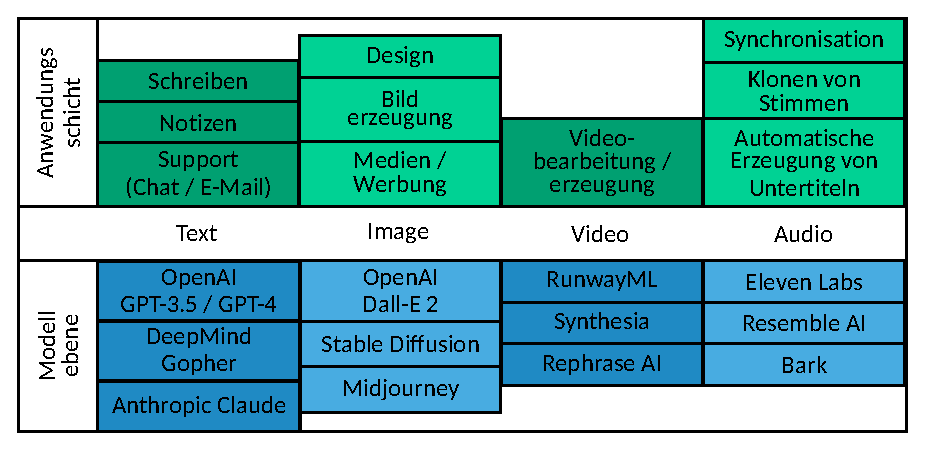
\includegraphics[width=\textwidth]{chapter/chapter_2/generative-ai-landscape.eps}
    \caption{Übersicht ausgewählter aktueller Systeme generativer KI nach \cite{sequoia-genai}.}
    \label{sec2:sota:subsec:fz-explainablity:fig:generative-ai-landscape}
\end{figure}

% \FloatBarrier

\paragraph{Einschränkungen}
Systeme generativer KI, wie z.B. das große Sprachmodell GPT-3 von OpenAI, sind bereits in der Lage realistische und höchst überzeugende Inhalte zu erzeugen.
Trotzdem unterliegen Systeme generativer KI einer Reihe an Einschränkungen, die sich potentiell auf ihre Fähigkeiten und Anwendungsfälle auswirken können.
Einige der wichtigsten Einschränkungen von Systemen generativer KI sind:
\begin{enumerate}
    \item \textbf{Mangelnde Transparenz und Erklärbarkeit}: Modelle generativer KI sind sog. Black-Boxen und bieten keinen Einblick in ihren Entscheidungsprozess \cite{explainable-ai-kobold}.
    Aufgrund dieser mangelnder Transparenz ist es nicht ersichtlich, wie ein Modell zu einer Entscheidung und zu einem Ergebnis kommt \cite{explainable-ai-kobold}.
    Resultat ist eine eingeschränkte Erklärbarkeit von Modellen.

    \item \textbf{Abhängigkeit von Trainingsdaten und ethische Bedenken}: Modelle generativer KI sind Produkte ihrer Trainingsdaten und daher stark von ihnen abhängig \cite{klinkhammer-genai}.
    Aufgrund dieser Abhängigkeit können sich Ungenauigkeiten aus den Trainingsdaten in den generierten Ergebnissen widerspiegeln \cite{klinkhammer-genai}.
    Des Weiteren sind diese Modelle zumeist speziell auf Bereiche angepasst und lassen sich nur schwer auf andere Bereiche anwenden, die nicht von den Trainingsdaten vorgesehen sind \cite{klinkhammer-genai}.
    Ein weiteres Problem generativer KI sind ethische Bedenken \cite{klinkhammer-genai}.
    Durch Voreingenommenheiten in den Trainingsdaten können Modelle selbst voreingenommene oder gar schädliche Inhalte erzeugen \cite{klinkhammer-genai}.

    %\item \textbf{Mangelndes Verständnis des Kontextes und Mehrdeutigkeit}: Modelle generativer KI haben, trotz Mechanismen, wie z.B. dem Selbstaufmerksamkeitsmechanismus, oft Probleme den Kontext eines Textes zu verstehen \cite{azumo-genai-power}.
    %Sie können deshalb keine komplexen Zusammenhänge erkennen und nachvollziehen.
    %Dies führt aufgrund der Mehrdeutigkeit von natürlicher Sprache zu Problemen in Bezug auf kontextabhängige Aussagen.
    %Generative KI hat Schwierigkeiten, die Mehrdeutigkeiten in einer Aufgabe zu trennen.
    %Dies kann zu ungenauen Ergebnissen mit unbeabsichtigten Bedeutungen führen.

    \item \textbf{Mangelndes Verständnis des Kontextes}:
    Die Länge des Kontextfensters eines Modells begrenzt die Menge an vorausgehendem Text, welches ein Modell bei der Generierung einer Antwort auf eine Eingabeaufforderung berücksichtigt \cite{v7labs-llm-limitations}.
    Informationen, die außerhalb dieses Kontextfensters liegen, werden unter Umständen nicht mehr berücksichtigt und können zu einem unvollständigen Verständnis des Textes oder zu kontextuell verfälschten Antworten führen \cite{v7labs-llm-limitations}.
    In Kombination mit den ausgewählten Trainingsdaten beeinflusst die Länge des Kontextfensters somit maßgeblich die Fähigkeiten des Modells den Kontext zu verstehen, langfristige Abhängigkeiten zu erfassen und kohärente Texte zu generieren \cite{v7labs-llm-limitations}.
\end{enumerate}

Trotz der bemerkenswerten Fähigkeit ansprechende und überzeugende Inhalte zu generieren, ist es wichtig die Einschränkungen und Grenzen generativer KI im Blick zu behalten, um so einen effektiven, verantwortungsbewussten und informierten Einsatz von generativer KI garantieren zu können.
Im Bereich der Forschung gibt es laufende Bemühungen und Weiterentwicklungen, um diese Einschränkungen und Grenzen zu adressieren, abzustellen, die Zuverlässigkeit von generativer KI zu verbessern, sowie Fähigkeiten von Systemen generativer KI weiter auszubauen.
Diese Bestrebungen können allgemein unter dem Begriff \enquote{Responsible AI} zusammengefasst werden, welche zum Ziel haben KI auf verantwortungsvolle Art und Weise zu entwickeln und die oben genannten Einschränkungen zu berücksichtigen \cite{gabler-responsible-ai}.

\subsubsection{Diskussion}
\label{sec2:sota:subsubsec:fz1:discussion}
In den ersten {\crefname{subsection}{Abschnitte}{Abschnitten}\cref{sec2:sota:subsubsec:gmaf,sec2:sota:subsubsec:mmfg,sec2:sota:subsubsec:graph-codes}} wurden zuerst grundlegende Technologien in Bezug auf das GMAF, welches das Bezugssystem dieser Arbeit darstellt, vorgestellt und detailliert erläutert.
Weiter wurden in \cref{sec2:sota:subsubsec:genai} grundlegende Techniken und Konzepte im Rahmen der generativen KI genannt und erklärt, sowie aktuelle Systeme generativer KI nach Kategorien gelistet.

Im Rahmen der Diskussion dieses Forschungsziels werden die Anwendungsmöglichkeiten der in \cref{sec2:sota:par:genai-systems} vorgestellten Systeme in Bezug auf das GMAF diskutiert.
Anhand dieser Diskussion wird dann eine fundierte Entscheidung getroffen, welche Systeme generativer KI für die Umgebung \enquote{Erklärbarkeit von MMIR mittels generativer KI} am besten geeignet sind.

Damit eine fundierte und informierte Entscheidung für die Auswahl von Systemen generativer KI getroffen werden kann, gilt es einige Kriterien zur Auswahl von Systemen zu beachten.
Wichtige Kriterien zur Auswahl eines Systems sind:
\begin{itemize}
    \item \textbf{Anpassungsmöglichkeiten}: Wie flexibel ist ein System?
    Ermöglicht es die Anpassung anhand Anforderungen besonderer Anwendungsfälle?
    \item \textbf{Kompatibilität und Integration}: Ist ein System mit der Programmiersprache oder der Umgebung des GMAF kompatibel?
    Bietet das System eine Schnittstelle, um eine einfache Integration des Systems in das GMAF zu ermöglichen?
    Bietet das System eine klare Dokumentation, um die Integration der Schnittstelle zu unterstützen?
    \item \textbf{Skalierbarkeit und Leistung}: Ist das System in der Lage größere Datenmengen zu verarbeiten?
    Kann es auf Anfrage zeitnah Ergebnisse generieren?
    \item \textbf{Kosten und Lizenzierung}: Einige Systeme bieten kostenfreie Nutzung oder berechnen die Kosten abhängig von der Nutzung, wiederum erfordern andere Systeme eine kommerzielle Lizenz zur Nutzung.
    Welche Lizenzbedingung oder Preise sind mit der Nutzung eines Systems verbunden?
\end{itemize}

Das Berücksichtigen dieser Kriterien in der Auswahl eines Systems generativer KI ermöglicht eine wohl informierte und fundierte Entscheidung über die Integration eines Systems in das GMAF und legt das Fundament für das Erreichen von Anforderungen und Zielen.
Daher wird zuerst die Auswahl eines Systems aus der Kategorie Image zur Bildgenerierung diskutiert.
Danach folgt eine Diskussion zur Auswahl eines Systems aus der Kategorie Text zur Textgenerierung.
Die Diskussion orientiert sich dabei jeweils nach den Systemen und nicht nach den oben genannten Kriterien.

\paragraph{Ausgewählte Systeme zur Bildgenerierung}
Zur Auswahl eines Systems zur Bildgenerierung stehen OpenAIs DALL·E 2, StabilityAIs Stable Diffusion und Midjourney.
Um einen besseren Eindruck zu den jeweiligen Modellen bzw. Systemen zu ermöglichen, wird für jedes System ein Bild anhand der Textbeschreibung bzw. Prompt \enquote{\textit{Beautiful Venice canals with gondolas and bridges, charming}} generiert.

% Prüfen, ob auch alle Aspekte abgedeckt werden ...
% Beispiele beifügen für die jeweiligen Systeme, um dem Leser besseren Eindruck zu ermöglichen

\textbf{Midjourney} ist eine generative KI, die auf Grundlage einer Textbeschreibung überzeugende und ästhetisch ansprechende Bilder erzeugen kann.
\cref{sec2:sota:subsubsec:fz1:discussion:fig:venice-midjourney} zeigt ein Beispiel für ein von Midjourney generiertes Bild.
\begin{figure}[htb]
    \centering
    \includegraphics[width=0.65\textwidth, keepaspectratio]{chapter/chapter_2/venice-midjourney.png}
    \caption{Beispiel für ein von Midjourney generiertes Bild anhand oben genannter Textbeschreibung \cite{reddit-venice-midjourney}.}
    \label{sec2:sota:subsubsec:fz1:discussion:fig:venice-midjourney}
\end{figure}
Um auf Midjourney zugreifen zu können, wird eine Anmeldung über den Onlinedienst Discord vorausgesetzt.
Weitere Voraussetzungen zum Nutzen Midjourneys sind das Hinzufügen und Beitreten des Discord-Servers von Midjourney und das Akzeptieren der allgemeinen Nutzungsbedingungen.
Sind diese Voraussetzungen erfüllt, kann Midjourney über Befehle im Discord-Chat gesteuert werden.
Bilder können über den Befehl /imagine und einer Textbeschreibung \textbf{prompt} erzeugt werden.
Midjourney bietet eine Reihe an Anpassungsmöglichkeiten seiner Prozesse, die gezielt durch Befehle, die in \cite{midjourney-docs} dokumentiert sind, vorgenommen werden können.
Midjourney bietet in einem begrenztem Testversuch ein initiales Guthaben von 25 Credits zum Erstellen von Bildern.
Sind diese Credits aufgebraucht, kann aus einer Reihe an unterschiedlichen, gestaffelten Mitgliedschaften (siehe \cite{midjourney-plans}), welche jeweils eigene Vorteile bieten, gewählt werden.
Eine Integration von Midjourney in eine andere Software ist aufgrund einer fehlenden Schnittstelle oder Anbindung bzw. Bibliothek nicht möglich.
Zwar gibt es Drittanbieter, die eine Schnittstelle bereitzustellen scheinen, allerdings verweist Midjourney in seinen allgemeinen Nutzungsbedingungen ausdrücklich, dass es keine Schnittstelle bereitstellt und Automatisierungen nicht duldet \cite{midjourney-tos}.

\textbf{Stable Diffusion} von StabilityAI ist eine quelloffene generative KI, die ebenfalls auf Grundlage einer Textbeschreibung Bilder erzeugen kann.
\cref{sec2:sota:subsubsec:fz1:discussion:fig:venice-stable-diffusion} zeigt ein Beispiel für ein von Stable Diffusion generiertes Bild.
\begin{figure}[htb]
    \centering
    \includegraphics[width=0.65\textwidth, keepaspectratio]{chapter/chapter_2/venice-stable-diffusion.png}
    \caption{Beispiel für ein von Stable Diffusion generiertes Bild anhand oben genannter Textbeschreibung.}
    \label{sec2:sota:subsubsec:fz1:discussion:fig:venice-stable-diffusion}
\end{figure}
Zugriff auf Stable Diffusion kann durch eine Installation auf einer lokalen Maschine oder durch das WebInterface DreamStudio erfolgen.
In beiden Fällen erfolgt der Zugriff durch ein WebInterface, in welchem eine Reihe an Anpassungsmöglichkeiten durch Einstellungen vorgenommen werden können.
%Eine lokale Installation ist im Rahmen dieser Arbeit ausgeschlossen, da für eine vernünftige Nutzung von Stable Diffusion eine Mindestanforderung von 10GB VRAM notwendig ist.
Aufgrund der hohen Rechenanforderungen benötigt eine lokale Installation von Stable Diffusion eine hohe Mindestanforderung an VRAM.
%10GB VRAM mind.
Auch Stable Diffusion bietet in einem begrenztem Testversuch ein initiales Guthaben von 25 Credits.
Sind diese Credits aufgebraucht, können für einen Mindestwert von 10 Euro Credits hinzugekauft werden.
Die Preise für die Generierung von Bildern sind abhängig von den gewählten Eigenschaften der Bilder und können in \cite{sd-pricing} eingesehen werden.
Eigenschaften können die Bildgröße, aber auch die Anzahl der Iterationen der Bildgenerierung sein.
Diese Einstellungen haben einen Einfluss auf die Qualität der generierten Bilder und folglich auch auf die Rechenintensität und beeinflussen dementsprechend die Preise zur Generierung von Bildern.
Eine Integration von Stable Diffusion ist durch eine offizielle REST (Representational State Transfer) \cite{rest} Schnittstelle möglich.
%Stable Diffusion ist lizenziert unter der CreativeML Open RAIL++-M Lizenz.
% Nur anmerken, dass es Schnittstelle gibt, oder noch OpenAPI anmerken?

\textbf{DALL·E 2} ist eine generative KI, die ebenfalls auf Grundlage einer Textbeschreibung Bilder erzeugen kann.
\cref{sec2:sota:subsubsec:fz1:discussion:fig:venice-dall·e} zeigt ein Beispiel für ein von DALL·E 2 generiertes Bild.
\begin{figure}[htb]
    \centering
    \includegraphics[width=0.65\textwidth]{chapter/chapter_2/venice-dall-e.png}
    \caption{Beispiel für ein von DALL·E 2 generiertes Bild anhand oben genannter Textbeschreibung.}
    \label{sec2:sota:subsubsec:fz1:discussion:fig:venice-dall·e}
\end{figure}
Zugriff auf DALL·E 2 erfolgt über ein WebInterface.
OpenAI bietet monatlich eine freie Anzahl an Credits, mit welchen Bilder erzeugt werden können.
Sind diese Credits aufgebraucht, kann für einen Mindestwert von 15 Dollar 115 Credits hinzugekauft werden.
Im Vergleich zu Stable Diffusion sind die Preise zur Bildgenerierung von DALL·E 2 nur von der Bildgröße abhängig (siehe \cite{openai-pricing}).
OpenAI bietet über eine Schnittstelle Zugriff auf DALL·E 2, sowie andere Modelle.
Diese Schnittstelle verfügt über eine wohl definierte Dokumentation, die in \cite{openai-api-doc} eingesehen werden kann.
Des Weiteren unterstützt OpenAI zur Integration seiner Modelle eine Reihe an Community-Bibliotheken für unterschiedliche Sprachen, darunter eine Anbindung der Schnittstelle für Java (siehe \cite{dall-e-java-api}).
Auch die Dokumentation zur Anbindung der Schnittstelle in Java unterstützt eine klare Dokumentation (siehe \cite{dall-e-java-api}).

Alle drei vorgestellten Systeme ermöglichen das Erzeugen von qualitativ hochwertigen Bildern.
Hinter allen drei Systemen stehen in Bezug auf die Bepreisung der Generation von Bildern sogenannte Credits.
Dabei bieten alle drei Systeme am Anfang eine gewisse Zahl an freien Credits.
Midjourney und Stable Diffusion vergeben beim Erstellen eines Kontos eine endliche Anzahl an Credits.
OpenAI hingegen vergibt ein anfängliches Guthaben von 5 Dollar und monatlich eine freie Anzahl an Credits, die jeden Monat zurückgesetzt werden.
Credits gelten allerdings nicht für die Schnittstelle von OpenAI und werden separat berechnet \cite{openai-dall-e-seperate-billing}.
Die Anzahl der Credits sind im Rahmen von OpenAI somit nicht von Belang.
Die Berechnung der Preise geschehen im Fall der Schnittstelle von OpenAI nutzungsbasiert und werden am Ende des Monats abgerechnet, anstatt einer monatlichen Zahlung wie im Fall von Midjourney.
Die Tatsache, dass Midjoruney keine Schnittstelle anbietet, disqualifiziert Midjourney für die Auswahl eines Systems zur Bildgenerierung im Rahmen dieser Arbeit.
Offen für die Auswahl bleiben StabilityAIs Stable Diffusion und OpenAIs DALL·E 2.
Ein Argument gegen Stable Diffusion ist, dass sobald Credits aufgebraucht sind, auch zum Anwenden der Schnittstelle neue Credits für einen Mindestwert von 10 Euro hinzugekauft werden müssen, was umgerechnet 1000 standardmäßig generierten Bildern entspricht.
Stable Diffusion setzt die Credits, im Gegensatz zu OpenAIs DALL·E 2, voraus, um die REST Schnittstelle nutzen zu können.
Ein Argument für OpenAIs DALL·E 2 ist die bestehende Java Anbindung für die Schnittstelle, die eine einfache Integration ermöglicht.
Im Rahmen dieser Arbeit wird für die folgende Modellierung und Implementierung Dall-E 2 als Vertreter zur Bildgenerierung ausgewählt.

\paragraph{Ausgewählte Systeme zur Textgenerierung}
Zur Auswahl eines Systems zur Textgenerierung stehen OpenAIs Sprachmodelle, wie GPT-3.5 und GPT-4, sowie Googles PaLM 2.
Die Anwendung der Systeme zur Textgenerierung werden an folgendem Beispiel demonstriert: \enquote{Auf meiner Reise durch die Städte Frankreichs ist mir in einem kleinen Dorf in einem Dialog mit einer Bewohnerin ein Satz aufgefallen, dessen Sinn sich mir nicht erschließen will. Sie sagte: \enquote{Tomber dans les pommes}. Wollte sie mir Pommes zum Essen anbieten?}

\textbf{Pathway Language Model 2 (PaLM 2)} \cite{google-blog-io-23} ist ein von Google entwickeltes und auf enormen Datenmengen trainiertes großes Sprachmodell \cite{google-palm2-techreport}.
PaLM 2 zeichnet sich durch Fähigkeiten, wie das Verstehen, Erzeugen und Übersetzen von natürlicher Sprache, das Erzeugen von Code, sowie aber auch durch logisches Denken aus \cite{google-blog-io-23,google-palm2-techreport}.
Einige der wichtigsten Merkmale von PaLM 2 ist das verbesserte Verarbeiten von Daten, das Unterstützen vieler Sprachen und verbessertes logisches Denken im Vergleich zum Vorgänger PaLM \cite{google-palm2-techreport}.
Ungeachtet dessen kann PaLM 2 von Zeit zu Zeit unvollständige oder gar fälschliche Erklärungen bereitstellen \cite{google-bard-faq}.
Die PaLM 2 Familie besteht aus vier verschiedenen Modellen, die sich jeweils in aufsteigender Größe voneinander unterscheiden: \textit{Gecko, Otter, Bison, Unicorn} \cite{google-blog-io-23}.
Die unterschiedlichen Größen ermöglichen eine große Bandbreite an Anwendungsmöglichkeiten \cite{google-blog-io-23}.
Kleinere Modelle, wie Gecko könnten z.B. in mobilen Endgeräten Anwendung finden \cite{google-blog-io-23}.
PaLM 2 befindet sich noch in der Entwicklung und Google bietet zum Zeitpunkt des Verfassens dieser Arbeit keine offizielle öffentliche Schnittstelle für PaLM 2 an \cite{google-palm-api-announcement}.
Eine Möglichkeit dennoch Zugriff auf PaLM 2 zu erhalten, ist über Vertex AI oder über eine Warteliste \cite{google-palm-api-vertex-ai-waitlist}.
Eine weitere Möglichkeit PaLM 2 zu nutzen, ist Bard \cite{google-bard}, Googles Pendant zu ChatGPT \cite{openai-chatgpt}.
Die Bepreisung für das Nutzen der Vertex AI Schnittstelle ist abhängig von der mit den Anfragen verbundenen Rechennutzung \cite{google-vertex-ai-pricing}.
Da sich die PaLM Schnittstelle noch in einer Entwicklungsphase bzw. Vorschauphase befindet, ist der Zugriff für Entwickler, sofern freigeschaltet, kostenfrei \cite{google-palm-api-faq}.
Andernfalls steht die Ankündigung der Bepreisung der PaLM API durch Google noch aus \cite{google-palm-api-faq}.
Folgender Textausschnitt zeigt die Antwort auf das oben genannte Beispiel.
\begin{tcolorbox}
    [enhanced,
     colback=white,
     colbacktitle=white,
     coltitle=black,
     title=Bard (PaLM 2),
     toptitle=1.5mm,
     bottomtitle=1.5mm,
     center title,
     segmentation style={solid},
     overlay = {
        \begin{tcbcliptitle}
            \node[anchor=north west] at (frame.north west) {
                \includegraphics[width=7mm]{chapter/chapter_2/bard-icon-240x240.png}
            };
        \end{tcbcliptitle}
    }
]
\textbf{Bard:} Nein, die Bewohnerin wollte dir keine Pommes anbieten. Die französische Redewendung „tomber dans les pommes“ bedeutet „sich übergeben“. Es ist eine gängige Redensart in Frankreich, die verwendet wird, um auszudrücken, dass jemand sich sehr schlecht fühlt und sich übergeben muss.

Die Redensart hat ihren Ursprung im 18. Jahrhundert und leitet sich von dem französischen Wort „pomme“ ab, das „Apfel“ bedeutet. Im 18. Jahrhundert glaubte man, dass Äpfel eine heilende Wirkung haben und bei Übelkeit und Erbrechen helfen können. Daher wurde die Redewendung „tomber dans les pommes“ verwendet, um auszudrücken, dass jemand sich so schlecht fühlt, dass er Äpfel essen muss.

Heute wird die Redensart „tomber dans les pommes“ immer noch verwendet, um auszudrücken, dass jemand sich sehr schlecht fühlt und sich übergeben muss. Es ist eine gängige Redensart in Frankreich und wird auch in anderen französischensprachigen Ländern verwendet.
\end{tcolorbox}
\medbreak

% Hier dann OpenAIs Sprachmodelle ansprechen und Eigenschaften nennen.

\textbf{GPT-3.5} \cite{openai-gpt-sep-2021} und \textbf{GPT-4} \cite{openai-gpt-sep-2021} sind von OpenAI entwickelte und ebenfalls auf enormen Datenmengen trainierte große Sprachmodelle.
Ähnlich wie PaLM 2 sind GPT-3.5 und GPT-4 in der Lage Text zu verstehen, Text zu erzeugen, Fragen zu beantworten und Übersetzungen oder Zusammenfassungen anzufertigen \cite{gpt3-paper}.
GPT-4 stellt die neuste Version der GPT Modellreihe dar und soll laut OpenAI besseres Textverständnis und eine höhere Leistung als die Vorgängermodelle liefern \cite{openai-gpt-4-announcement}.
Da OpenAI keine genauen Spezifikationen zu GPT-3.5 und GPT-4 veröffentlicht hat, ist die genaue Anzahl der Parameter in GPT-3.5 bzw. GPT-4 nicht bekannt, aber laut Gerüchten soll sich die Anzahl auf 175 Milliarden bzw. 1 Billion Parameter belaufen \cite{decoder-gpt-4-parameter-count}.
Im Vergleich dazu umfasst das Vorgängermodell GPT-3, von welchem GPT-3.5 nur eine optimierte Version ist, nur 175 Milliarden Parameter \cite{gpt3-paper}.
Eine der neusten Funktionen von GPT-4 ist die Eingabe und Verarbeitung von Bildern, anhand welcher es Erklärungen generieren können soll \cite{openai-gpt-4-announcement}.
Dies macht GPT-4 zu einem echten multimodalen Modell, welches mehrere Arten von Eingaben akzeptieren kann \cite{openai-gpt-4-announcement}.
Bildeingaben sind aber nach wie vor in einer begrenzten Alpha Testphase und nicht unmittelbar verfügbar \cite{openai-gpt-4-announcement}.
OpenAI bietet über eine REST Schnittstelle einfachen Zugriff auf die Sprachmodelle, wie GPT-3.5 und GPT-4, sowie Derivate, wie z.B. GPT-3.5-Turbo-(4k/16k).
Unterschiede in diesen Derivaten liegen in der Größe des Kontextes, also der Länge an Textzeichen, die ein Modell bei der Generierung berücksichtigt.
Die für die Sprachmodelle angebotene Schnittstelle ist die gleiche Schnittstelle wie die für DALL·E 2 und bietet ebenfalls eine umfassende Dokumentation (siehe \cite{openai-api-doc}).
Diese Dokumentation bietet nützliche Information, Leitfaden zur Nutzung, Beispiele für Quellcode und Beschreibungen für effektives Nutzen der Schnittstelle.
Seit dem 6. Juli 2023 erlaubt OpenAI den Zugriff auf das Sprachmodell GPT-4-8k für alle Anwender der Schnittstelle, die einen Verlauf erfolgreich abgeschlossener Zahlungen aufweisen \cite{openai-gpt4-access}.
Die Bepreisung hängt dabei, sehr ähnlich zu PaLM 2, von der Anzahl an der in der Anfrage gesendeten Zeichen, sowie der in der Antwort enthaltenen Zeichen ab, und kann in \cite{openai-pricing} eingesehen werden.
Folgender Textausschnitt zeigt die Antwort auf das oben genannte Beispiel.
\begin{tcolorbox}
    [enhanced,
     colback=white,
     colbacktitle=white,
     coltitle=black,
     title=ChatGPT (GPT-3.5),
     toptitle=1.5mm,
     bottomtitle=1.5mm,
     center title,
     breakable,
     segmentation style={solid},
     overlay unbroken app ={
        \begin{tcbcliptitle}
            \node[anchor=north west] at (frame.north west) {
                \includegraphics[width=7mm]{chapter/chapter_2/openai-icon-240x240.png}
            };
        \end{tcbcliptitle}
    },
    overlay first app ={
        \begin{tcbcliptitle}
            \node[anchor=north west] at (frame.north west) {
                \includegraphics[width=7mm]{chapter/chapter_2/openai-icon-240x240.png}
            };
        \end{tcbcliptitle}
    }
]
\textbf{ChatGPT:} Nein, der Satz "Tomber dans les pommes" bedeutet nicht, dass die Bewohnerin dir Pommes zum Essen anbieten wollte. Tatsächlich ist es eine französische Redewendung, die einen Zustand beschreibt, in dem jemand ohnmächtig wird oder in Ohnmacht fällt. Die wörtliche Übersetzung ist "in die Äpfel fallen", aber im übertragenen Sinne bedeutet es, dass jemand kollabiert oder bewusstlos wird.

Diese Redewendung wird umgangssprachlich verwendet und ist im Französischen sehr geläufig, um einen plötzlichen Zustand der Bewusstlosigkeit oder des Zusammenbruchs zu beschreiben. Also, die Bewohnerin wollte dir keine Pommes anbieten, sondern sprach darüber, dass jemand ohnmächtig wird.
\tcbline
\textbf{Benutzer:} Sehr interessant, vielen Dank!
\tcbline
\textbf{ChatGPT:} Gern geschehen!
\end{tcolorbox}

Verglichen mit GPT-3.5 bietet GPT-4 grundlegend verbesserte Funktionen und Fähigkeiten \cite{openai-gpt-4-announcement}.
Ein weiterer Vergleich verbleibt somit zwischen OpenAIs Sprachmodellen GPT-3.5 und GPT-4, sowie Googles PaLM 2.

Ein grundlegendes Problem von Sprachmodellen ist, dass sie zu Halluzinationen neigen.
Es ist wichtig zu verstehen, dass wenn große Sprachmodelle auf enormen Datenmengen trainiert werden, sie die in diesen Daten enthaltenen statistische Muster und Strukturen erlernen \cite{basel-ml-arch}.
Als solches sind sie in der Lage Sätze oder Texte zu generieren, die kohärent wirken, ohne dabei wirklich ein wahres Verständnis des Textes oder ein Bewusstsein zu besitzen \cite{basel-ml-arch}.
Dies kann zu faktisch falschen oder unsinnigen Texterzeugnissen, auch Halluzinationen genannt, führen und sind Resultat von mangelndem Kontext und Textverständnis. \cite{sabre-pc-ai-hallucinations}.
Dieses Problem wird verstärkt durch veraltetes Wissen.
So gilt für die meisten Sprachmodelle von OpenAI, auch GPT-4, dass ihre Trainingsdaten respektive ihr Wissen nach September 2021 abrupt enden \cite{openai-gpt-sep-2021}.
Dies ist für viele Anwendungsfälle dieser Sprachmodelle eine einschneidende Einschränkung, besonders für den Aspekt der Erklärbarkeit.
Ungeachtet dessen sind alle vorgestellten Sprachmodelle nach wie vor von Natur aus Black-Boxes und weisen somit nur bedingt Erklärbarkeit auf.
Ein Argument für GPT-4 oder PaLM 2 ist, dass sie im Vergleich zu ihren Vorgängern jeweils eine wesentliche Verbesserung darstellen.
Eine besonders interessante Eigenschaft von PaLM 2 ist der Fokus auf Multilingualität, d.h. PaLM 2 wurde mit Daten in vielen Sprachen trainiert \cite{google-palm2-techreport}.
Jedoch ist ihr Zugang entweder zur Zeit nicht vorhanden oder kann nur über eine Warteliste angefragt werden.
Seit dem 6. Juli 2023 erlaubt OpenAI den Zugriff auf das Sprachmodell GPT-4-8k für alle Anwender der Schnittstelle, die einen Verlauf erfolgreich abgeschlossener Zahlungen aufweisen \cite{openai-gpt4-access}.
Ein Argument für GPT-3.5 ist hingegen die Schnelligkeit im Vergleich zu GPT-4 und ein weitaus einfacher Zugriff über die Schnittstelle, die bereits über eine Anbindung für Java verfügt.
Im Rahmen dieser Arbeit wird für die folgende Modellierung und Implementierung GPT-3.5 / 4 als Vertreter zur Textgenerierung ausgewählt.

\paragraph{Schlussfolgerung}
Anhand der Erkenntnisse der beiden Diskussionen zur Wahl von Systemen zur Bild-, sowie Textgenerierung, fällt die Wahl eines Systems zur Bildgenerierung auf OpenAIs DALL·E 2, sowie die Wahl eines Systems zur Textgenerierung auf das Sprachmodelle GPT-3.5 und seiner Derivate, sowie eventuell auf andere von OpenAI angebotenen Sprachmodelle.
Diese Entscheidungen liegen in den folgenden Eigenschaften begründet:
\begin{itemize}
    \item Einfache Integration durch die offiziell von OpenAI unterstützte Community Bibliothek \enquote{OpenAI-Java} \cite{dall-e-java-api} für Java.
    \item Beide Systeme, DALL·E 2 und die GPT-Sprachmodelle, werden bereitgestellt durch eine einzige Plattform: OpenAI.
    \item Zahlung einfach und flexibel an einen einzigen Anbieter.
    Zudem muss nur für das gezahlt werden, was wirklich genutzt wird, \textit{Only pay for what you use}, anstatt einer monatlichen Fixzahlung.
\end{itemize}
Die Wahl der primären Systeme liegt somit bei den oben genannten Systemen, deren Einsatz im weiteren Verlauf dieser Arbeit verfolgt wird.
Unabhängig von der Wahl der primären Systeme verbleiben die Systeme PaLM 2 oder Stable Diffusion weiterhin als optionale Kandidaten, die ebenfalls integriert werden könnten.

Die ausgewählten Systeme bieten umfassende Möglichkeiten zur Bild- und Textgenerierung.
Jedoch existiert keine Benutzungsschnittstelle im GMAF, die geeignete Interaktionsmöglichkeiten für Systeme generativer KI ermöglicht.
Dies führt zu einer weiteren, zweiten Herausforderung im Rahmen dieses Forschungsziels.

\begin{tcolorbox}[minipage, breakable, colback=white, arc=0pt, outer arc=0pt]
    \textbf{Offene Herausforderung OH 1.2 - Benutzungsschnittstelle} \\
    Sollen diese Systeme im Rahmen des GMAF sinnvoll eingesetzt werden, um Erklärungen generieren zu können, so müssen Anwendern des GMAF durch eine Benutzungsschnittstelle geeignete Interaktionsmöglichkeiten mit diesen Systemen geboten werden.
\end{tcolorbox}

Die offene Herausforderung \openissue{sec2:sota:oi:1.2}{OH 1.2} hat in Bezug auf dieses Forschungsziel einen einschränkenden Charakter.
Das Forschungsziel bezieht sich in erster Linie auf Erklärbarkeit von MMIR im Allgemeinen und hat hierfür eine Reihe an existierenden Systemen generativer KI untersucht und vorgestellt.
Die offene Herausforderung begrenzt hingegen das Augenmerk auf die Problematik, dass Anwender des GMAF die ausgewählten Systeme generativer KI sinnvoll nutzen sollen, hierfür im GMAF aber keine Benutzungsschnittstelle mit geeigneten Interaktionsmöglichkeiten besteht.

Die offene Herausforderung \textbf{OH 1.2} wird im Rahmen einer Modellierung, sowie Implementierung ebenfalls in jeweils \hyperref[sec3:model:subsec:fz-explainability]{FZ 1.2/TB} und \hyperref[sec4:impl:subsec:fz-explainability]{FZ 1.3/I} angesprochen und untersucht.

Im nächsten Abschnitt werden die im Rahmen dieses Forschungsziels identifizierten offenen Herausforderungen zusammengefasst.

\paragraph{Offene Herausforderungen}
\label{sec2:sota:par:fz1:open-challenges}
In \cref{sec2:sota:subsubsec:gmaf,sec2:sota:subsubsec:mmfg,sec2:sota:subsubsec:graph-codes} wurden Technologien in Bezug auf das GMAF vorgestellt.
Es konnte festgestellt werden, dass der Ansatz MMFGs bzw. Graph Codes erklärbar zu machen, sehr statistisch und rein mathematischer Natur ist.
Eine Verbesserung bzw. einen alternativen Ansatz, um MMFGs bzw. Graph Codes erklärbar machen zu können, verspricht der Einsatz von Systemen generativer KI.
Dies führt zur ersten offenen Herausforderung \textbf{OH 1.1} und der Frage \enquote{Wie kann generative KI eingesetzt werden, um Erklärbarkeit zu erreichen?}.
% Eventuell Unterschied zwischen Erklärbarkeit von generativer KI und Erklärbarkeit durch generative KI hervorheben?
Es gilt daher im Rahmen der Umgebung \enquote{Erklärbarkeit von MMIR mittels generativer KI} zu ermitteln, wie Systeme generativer KI genutzt werden können, um Erklärbarkeit zu erreichen bzw. Erklärungen zu generieren.

Im weiteren Verlauf wurden im \cref{sec2:sota:subsubsec:genai} grundlegende Technologien, Techniken und Eigenschaften beschrieben und eine Reihe an Systemen generativer KI vorgestellt.
Aus dieser Reihe an Systemen wurde in \cref{sec2:sota:subsubsec:fz1:discussion} eine Auswahl an Systemen getroffen, deren Einsatz im weiteren Verlauf dieser Arbeit verfolgt werden.
Die in diesem Abschnitt vorgestellten und ausgewählten Systeme bieten umfassende Möglichkeiten zur Bild- und Textgenerierung.
Sollen diese Systeme im Rahmen des GMAF sinnvoll eingesetzt werden, um Graph Codes erklärbar zu machen, so müssen Anwendern des GMAF durch eine Benutzungsschnittstelle geeignete Interaktionsmöglichkeiten mit diesen Systemen geboten werden.
Es konnte festgestellt werden, dass das GMAF für seine Anwender keine Interaktionsmöglichkeiten mit Systemen generativer KI bietet.
Dies führt zur zweiten offenen Herausforderung \textbf{OH 1.2} und der Frage \enquote{Wie muss eine Benutzungsschnittstelle beschaffen sein, um geeignete Interaktionsmöglichkeiten mit Systemen generativer KI zu ermöglichen?}.
%Es gilt daher die Funktionen dieser Systeme für die Umgebung \enquote{Erklärbarkeit von MMIR mittels generativer KI} im Rahmen des GMAF und in einem eigens dafür bestimmten Programm oder als Erweiterung in das GMAF anhand von Anwendungsfällen zu integrieren.
Es gilt daher anhand von Anwendungsfällen geeignete Schnittstellen zur Interaktion mit den in diesem Abschnitt vorgestellten Systemen generativer KI für die Umgebung \enquote{Erklärbarkeit von MMIR mittels generativer KI} im Rahmen des GMAF in einem eigens dafür bestimmten Programm oder als Erweiterung in das GMAF umzusetzen.

Die beiden offenen Herausforderungen \textbf{OH 1.1} und \textbf{OH 1.2} werden im Rahmen einer Modellierung durch das Forschungsziel FZ 1.2/TB angesprochen und durch das Forschungsziel 1.3/I im Rahmen einer prototypischen Implementierung untersucht.
Forschungsziel 1.4/E wird sich der Evaluierung der in diesen Kapiteln erlangten Forschungsergebnissen widmen.

\clearpage

\subsection{FZ 2.1/O Integration generativer KI in das GMAF}
\label{sec2:sota:subsec:fz-integration}
Dieser Abschnitt gibt einen Überblick über ausgewählte Ergebnisse und Erkenntnisse aus der Forschung im Bereich der Integration von Systemen generativer KI und deckt technische Aspekte ab, die sich auf die zweite Problembeschreibung beziehen.
\cref{sec2:sota:subsubsec:gc-capabilities-integration} widmet sich den Integrationsmöglichkeiten von Graph Codes.
Weiter befasst sich \cref{sec2:sota:subsubsec:genai-capabilities-integration} mit den Integrationsmöglichkeiten von Systemen generativer KI.

\subsubsection{Integrationsmöglichkeiten von Graph Codes}
\label{sec2:sota:subsubsec:gc-capabilities-integration}
Dieser Abschnitt befasst sich mit den Integrationsmöglichkeiten von Graph Codes.
Wie bereits in \cref{sec2:sota:subsubsec:graph-codes} beschrieben, sind Graph Codes eine Technologie zur effizienten und effektiven Darstellung und Verarbeitung von Merkmalen im GMAF.
Als solches ist eine Integration von Graph Codes im Rahmen des GMAF bereits gegeben.
Diese Integration bietet im Rahmen des GMAF folgende Komponenten:
\begin{itemize}
    \item \textit{GraphCode} bietet eine Implementierung der zweidimensionalen Darstellung von Merkmalen und ermöglicht Zugriff auf das Wörterbuch eines Graph Codes.
    \item \textit{GraphCodeCollection} bietet eine Reihe an Operationen, wie z.B. die Vereinigung oder Subtraktion von Graph Codes an.
    \item \textit{GraphCodeGenerator} ist eine Implementierung, die das Erstellen eines Graph Codes aus einem MMFG ermöglicht.
    \item \textit{GraphCodeIO} bietet eine Reihe an nützlichen Operationen zum Import oder Export von Graph Codes aus oder in Dateien.
    \item \textit{GraphCodeMetric} bietet eine Implementierung der in \cref{sec2:sota:par:gc-similiarity} beschriebenen Metrik zur Ähnlichkeit von Graph Codes.
\end{itemize}

Die grundsätzliche Darstellungsform eines Graph Codes erfolgt im textbasierten Dateiübertragungsformat JSON (JavaScript Object Notation) und kann somit leicht von Menschen, aber auch Maschinen gelesen und verarbeitet werden.
\cref{sec2:sota:subsec:fz2:lst:gc-ex-json} zeigt das Beispiel des Graph Codes $GC_{ex}$ in JSON-Format.
\begin{lstlisting}[
    language=json,
    firstnumber=1,
    label={sec2:sota:subsec:fz2:lst:gc-ex-json},
    captionpos=b,
    caption={Beispiel des Graph Codes $GC_{ex}$ im JSON-Format.}
]
{
  "dictionary": [
    "root-image",
    "person",
    "body",
    "arm",
    "watch"
  ],
  "collectionElements": [],
  "matrix": [
    [1,1,0,0, 0],
    [0,1,1,0, 0],
    [0,0,1,1, 0],
    [0,0,0,1,17],
    [0,0,0,0, 2]
  ]
}
\end{lstlisting}

Dieses Beispiel zeigt, wie die Informationen eines Graph Codes, wie z.B. das Wörterbuch oder die Wertungsmatrix, als ein Objektgraph bestehend aus mehreren Paaren von Schlüssel und Werten im Syntax \textbf{Schlüssel : Wert} dargestellt werden.
Im Falle der Paare aus Schlüsseln und Werten stellen Schlüssel immer eine Zeichenfolge, wie \enquote{dictionary}, \enquote{collectionElements} oder \enquote{matrix} dar, während Werte Zahlen, Strings, Arrays oder wiederum Objekte sein können.
Die Elemente \enquote{dictionary} und \enquote{collectionElements} haben jeweils Arrays als Werte, in welchen eine Menge an Bezeichnern bzw. Graph Codes enthalten sein können.
Da die gesamte Darstellung eines Graph Codes im JSON-Format wiederum ein Objekt ist, kann \enquote{collectionElements} eine Menge bzw. Sammlung an Darstellungen von Graph Codes enthalten.
Auf diese Weise kann eine rekursive Darstellung von Graph Codes erreicht werden.
Das Element \enquote{matrix} hat ebenfalls ein Array als Wert.
Da allerdings die Adjazenzmatrix eine zweidimensional Matrix ist, sind die Werte im Array wiederum Arrays aus ganzen Zahlen mit einer Länge, die äquivalent zu Größe des Wörterbuchs ist.
Das GMAF integriert bereits für die Verarbeitung und Operationen mit JSON die GSON \cite{gson} Bibliothek von Google ein.

Auch wenn Systeme wie GPT-3.5 oder GPT-4 und PaLM 2 in der Lage sind Daten im JSON-Format in Textform zu verarbeiten, so bleibt jedoch offen, wie die Informationen aus einem Graph Code und die damit assoziierten Informationen in die Eingabe für ein System generativer KI überführt werden kann, und welche Eigenheiten berücksichtigt werden müssen.
Dies führt zu einer ersten offenen Herausforderung im Rahmen dieses Forschungsziels.
\begin{tcolorbox}[minipage, colback=white, colframe=black, arc=0pt, outer arc=0pt]
    \textbf{Offene Herausforderung OH 2.1 - Transformieren von Graph Codes} \\
    Umwandlung von Graph Codes in eine passende Eingabeform für Systeme generativer KI.
\end{tcolorbox}

Die offene Herausforderung \openissue{sec2:sota:oi:2.1}{OH 2.1} hat in Bezug auf dieses Forschungsziel einen einschränkenden Charakter.
Das Forschungsziel bezieht sich auf die Integrationsmöglichkeiten von Graph Codes und stellt eine Reihe an Komponenten vor, die mit Graph Codes assoziiert sind und im GMAF implementiert sind.
Die offene Herausforderung begrenzt hingegen das Augenmerk auf die Problematik, dass die vorgestellten und bereits im GMAF implementierten Komponenten, keine Möglichkeiten zur Transformation der in Graph Codes gespeicherten Informationen in eine passende Eingabeform für Systeme generativer KI bieten.

Die offene Herausforderung \textbf{OH 2.1} wird im Rahmen einer Modellierung, sowie Implementierung in jeweils \hyperref[sec3:model:subsec:fz-integration]{FZ 2.2/TB} und \hyperref[sec4:impl:subsec:fz-integration]{FZ 2.3/I} angesprochen und untersucht.

\subsubsection{Integrationsmöglichkeiten von Systemen generativer KI}
\label{sec2:sota:subsubsec:genai-capabilities-integration}
Dieser Abschnitt befasst sich mit den Möglichkeiten der Integration der in \cref{sec2:sota:subsubsec:fz1:discussion} ausgewählten Systeme generativer KI.
Dies sind in erster Linie die Systeme, GPT-3.5/4 und Dall-E, die von OpenAI entwickelt wurden.
OpenAI bietet zur Übersicht eine Plattform für seine Produkte an.
Diese Plattform umfasst neben den Produkten auch Anleitungen, Beispiele und Tipps zu bewährten Praktiken zu diesen Produkten und beschreibt eine Reihe an Möglichkeiten zur Integration seiner Produkte.
Diese Integrationsmöglichkeiten umfassen:
\begin{itemize}
    \item Eine Schnittstelle (API), die es Entwicklern ermöglicht Modelle in ihre eigene entwickelte Software zu integrieren und aufzurufen.
    \item Unterstützte Systeme zur Softwareentwicklung (SDKs) in vielen Programmiersprachen, die u. a. von OpenAI bereitgestellt werden, oder von Mitgliedern der Community in anderen, nicht offiziell von OpenAI unterstützten Programmiersprachen entwickelt wurden \cite{openai-community-library}.
    \item Online-Dienste, die es Entwicklern ermöglichen Modelle ohne eigens entwickelte Software zu verwenden.
    Beispiele für diese Online-Dienste sind ChatGPT, Dall-E, Tokenizer oder ein Textklassifikator für KI.
    % https://platform.openai.com/tokenizer
    % https://platform.openai.com/ai-text-classifier
    \item Cloud-Dienste, die es Entwicklern ermöglichen Modelle ohne eigene Infrastruktur zu verwenden \cite{openai-cloud-services}.
\end{itemize}
Im nächsten Abschnitt wird gesondert auf die Schnittstelle und die Systeme zur Softwareentwicklung eingegangen.
Im darauffolgenden \cref{sec2:sota:par:tokenizer} werden dann weitere interessante Werkzeuge im Rahmen der Schnittstelle von OpenAI besprochen und Aspekte hervorgehoben.

\paragraph{API}
\label{sec2:sota:par:api}
Eine Schnittstelle (engl. \textbf{A}pplication \textbf{P}rogramming \textbf{I}nterface) ermöglicht Entwicklern die Kommunikation zwischen Softwareanwendungen umzusetzen.
Eine API definiert und stellt Funktionen bereit, die Entwickler verwenden können, um Softwareanwendungen miteinander zu verbinden.
Funktionen können das Auslesen und Schreiben von Daten, oder Ausführen von Aktionen in einer anderen Anwendung sein.
Auf diese Weise ermöglicht eine Schnittstelle den Zugriff auf Funktionen einer Anwendung, ohne dass diese in einer Anwendung selbst neu geschrieben bzw. programmiert werden müssen.

Die API von OpenAI kann praktisch auf jede Aufgabe angewendet werden, die das Verstehen oder Erzeugen von natürlicher Sprache betrifft und erfordert \cite{openai-docs-intro}.
Des Weiteren kann die API auch verwendet werden, um Bilder zu erzeugen, zu bearbeiten oder Sprache in Text zu konvertieren \cite{openai-docs-intro}.
Die API von OpenAI bietet Zugriff auf eine Reihe von Modellen, die unterschiedliche Fähigkeiten und Preise aufweisen \cite{openai-docs-intro}.

Die Schnittstelle von OpenAI wird durch eine RESTful (Representational State Transfer) Schnittstelle bereitgestellt.
REST-Schnittstellen sind eine der prominenteste Arten von APIs \cite{postman-state-of-api-2023}, die eine Reihe an Konventionen verwenden, um die Verarbeitung und Übertragung von Informationen zu gewährleisten.
Diese RESTful Schnittstelle wird spezifiziert über eine OpenAPI Spezifikationen \cite{openai-openapi-spec}, die die Funktionen der OpenAI Schnittstelle genaustens dokumentiert.
OpenAPI ist eine auf dem Architekturstil REST basierende Spezifikationssprache für die Beschreibung der Struktur, der Reihenfolge und des Verhaltens von APIs.
Diese Spezifikation wird für gewöhnlich in YAML oder JSON geschrieben und kann, neben der Dokumentation einer API, auch dazu verwendet werden, um mit spezialisierten Programmen, wie z.B. Swagger Codegen \cite{swagger}, automatisch Quellcode in einer spezifischen Programmiersprache zu generieren.
% https://swagger.io/tools/swagger-codegen/
Für die Programmiersprache Java wird diese Spezifikation bereits durch die SDK bzw. Bibliothek OpenAI-Java \cite{dall-e-java-api} abgedeckt.

Die API von OpenAI bietet Zugriff auf folgende Endpunkte:
\begin{enumerate}
    \item /v1/completions
    \item /v1/chat/completions
    \item /v1/edits
    \item /v1/images/generations
    \item /v1/images/edits
    \item /v1/images/variations
    \item /v1/embeddings
    \item /v1/audio/transcriptions
    \item /v1/audio/translations
    \item /v1/files
    \item /v1/fine-tunes
    \item /v1/moderations
\end{enumerate}
Im Rahmen dieser Arbeit sind nur die Endpunkte 2 und 4 zur Generierung von Text bzw. Bildern von Interesse.
In \cite{openai-api-doc} wird eine genaue Dokumentation, mitsamt Beispielen für diese Endpunkte beschrieben.

Eine Anfrage an den Endpunkt \textbf{/chat/completions/} nimmt als Eingabe eine Liste an Nachrichten in Form einer Unterhaltung zwischen verschiedenen Parteien.
Eine Nachricht besteht dabei aus einem Wertepaar \textbf{Rolle} : \textbf{Inhalt}.
Beide Werte sind notwendige Parameter einer Anfrage an diesen Endpunkt.
Der Parameter \textit{Rolle} kann einen von drei Werten annehmen: \textit{System}, \textit{Assistant}, \textit{User} \cite{openai-chat-compl-roles}.
Über den Endpunkt liefert das Modell eine Antwort auf diese Unterhaltung.

Eine Anfrage an den Endpunkt \textbf{/images/generations/} nimmt als Eingabe eine Eingabeaufforderung bzw. Prompt.
Das Modell generiert anhand dieser Prompt ein oder mehrere Bilder und liefert diese über den Endpunkt als Antwort zurück.

Die in diesem Abschnitt vorgestellte Schnittstelle mit all ihren Endpunkten bietet bereits umfassende Möglichkeiten zur Generierung von Text und Bildern.
Allerdings gibt es keine bestehende Integration dieser Systeme generativer KI im GMAF.
Dies führt zu zweiten, offenen Herausforderung im Rahmen dieses Forschungsziels.
\begin{tcolorbox}[minipage, colback=white, colframe=black, arc=0pt, outer arc=0pt]
    \textbf{Offene Herausforderung OH 2.2 - Integration generativer KI} \\
    Zum Zeitpunkt des Verfassens dieser Arbeit existiert keine Integration der von OpenAI angebotenen Systeme generativer KI im GMAF.
\end{tcolorbox}

Die offene Herausforderung \openissue{sec2:sota:oi:2.2}{OH 2.2} hat in Bezug auf dieses Forschungsziel einen konkretisierenden Charakter.
Das Forschungsziel bezieht sich auf die Integration von Systemen generativer KI und stellt hierfür die Schnittstelle und die darin spezifizierten Endpunkte genauer vor.
Die offene Herausforderung bezieht sich auf die Integration und Interaktion mit dieser Schnittstelle und ihren Endpunkten und verdeutlicht, dass es im GMAF keine Integration dieser Systeme existiert.

Die offene Herausforderung \textbf{OH 2.1} wird im Rahmen einer Modellierung, sowie Implementierung ebenfalls in jeweils \hyperref[sec3:model:subsec:fz-integration]{FZ 2.2/TB} und \hyperref[sec4:impl:subsec:fz-integration]{FZ 2.3/I} angesprochen und untersucht.

\paragraph{Tokenizer}
\label{sec2:sota:par:tokenizer}
Neben der Schnittstelle bietet OpenAI eine Reihe an Werkzeugen bzw. Online-Diensten an.
Eines dieser Werkzeuge ist der Tokenizer.
Die GPT-Modellreihe benutzt zum Verarbeiten von Text sogenannte Tokens \cite{openai-tokenizer}.
Tokens stellen häufige im Text vorkommende Zeichenfolgen dar \cite{openai-tokenizer}.
Die GPT-Modelle verstehen die statistischen Beziehungen zwischen diesen Token und sind anhand dieser Beziehungen und der bereits bestehenden Folge an Token im Text in der Lage das nächste Token im Text zu erzeugen \cite{openai-tokenizer}.
Ein abgewandeltes Beispiel für eine Tokenaufteilung ist im folgenden Text einsehbar:

\enquote{\sethlcolor{tok1}\hl{Multiple}\sethlcolor{tok2}\hl{ models}\sethlcolor{tok3}\hl{,}\sethlcolor{tok4}\hl{ each}\sethlcolor{tok5}\hl{ with}\sethlcolor{tok1}\hl{ different}\sethlcolor{tok2}\hl{ capabilities}\sethlcolor{tok3}\hl{ and}\sethlcolor{tok4}\hl{ price}\sethlcolor{tok5}\hl{ points}\sethlcolor{tok1}\hl{.}\sethlcolor{tok2}\hl{ Prices}\sethlcolor{tok3}\hl{ are}\sethlcolor{tok4}\hl{ per}\sethlcolor{tok5}\hl{ }\sethlcolor{tok1}\hl{1}\sethlcolor{tok2}\hl{,}\sethlcolor{tok3}\hl{000}\sethlcolor{tok4}\hl{ tokens}\sethlcolor{tok5}\hl{.}\sethlcolor{tok1}\hl{ You}\sethlcolor{tok2}\hl{ can}\sethlcolor{tok3}\hl{ think}\sethlcolor{tok4}\hl{ of}\sethlcolor{tok5}\hl{ tokens}\sethlcolor{tok1}\hl{ as}\sethlcolor{tok2}\hl{ pieces}\sethlcolor{tok3}\hl{ of}\sethlcolor{tok4}\hl{ words}\sethlcolor{tok5}\hl{,}\sethlcolor{tok1}\hl{ where}\sethlcolor{tok2}\hl{ }\sethlcolor{tok3}\hl{1}\sethlcolor{tok4}\hl{,}\sethlcolor{tok5}\hl{000}\sethlcolor{tok1}\hl{ tokens}\sethlcolor{tok2}\hl{ is}\sethlcolor{tok3}\hl{ about}\sethlcolor{tok4}\hl{ }\sethlcolor{tok5}\hl{750}\sethlcolor{tok1}\hl{ words}\sethlcolor{tok2}\hl{.}\sethlcolor{tok3}\hl{ This}\sethlcolor{tok4}\hl{ paragraph}\sethlcolor{tok5}\hl{ is}\sethlcolor{tok1}\hl{ }\sethlcolor{tok2}\hl{49}\sethlcolor{tok3}\hl{ tokens}\sethlcolor{tok4}\hl{.}} Encoding: \textit{(cl100k\_base)} \cite{openai-model-tiktoken}

Die Aufteilung der Zeichenfolgen in Tokens ist abhängig vom jeweiligen Modell und kann in \cite{openai-model-tiktoken} eingesehen werden.
Die Aufteilung eines Textes in Tokens ist deshalb interessant, da durch dieses Werkzeug die Anzahl der Tokens bestimmt werden kann.
In Kombination dieser Information und der Information zur Bepreisung kann ein potentielles Optimierungspotenzial in Bezug auf die Anzahl der Tokens und somit auch der Bepreisung ausgeschöpft werden.

Der Online-Dienst Tokenizer von OpenAI ist offiziell durch die für Python konzipierte Bibliothek \enquote{Tiktoken} \cite{openai-python-tiktoken} oder inoffiziell durch die für Java konzipierte Bibliothek \enquote{JTokkit} \cite{openai-java-jtokkit} als Schnittstelle für die Tokenisierung von Text verfügbar.

\subsubsection{Diskussion}
\label{sec2:sota:subsubsec:fz2:discussion}
In diesem Abschnitt wurden die Möglichkeiten der Integration von Graph Codes, sowie den von OpenAI angebotenen Systemen generativer KI behandelt.

In Bezug auf die Integrationsmöglichkeiten von Graph Codes konnte eine Übersicht über die vom GMAF gebotenen Komponenten, die eine entscheidende Rolle in der Technik der Graph Codes spielen, zusammengestellt werden.
Es wurde weiterhin bestimmt, dass die Darstellungsform der in Graph Codes enthaltenen Informationen im JSON-Format erfolgt.
Diese Darstellungsform kann insbesondere von aktuellen Systemen generativer KI effizient und effektiv eingelesen werden.

In Bezug auf die Integrationsmöglichkeiten der von OpenAI entwickelten Systemen generativer KI konnte eine Übersicht über die von OpenAI bereitgestellte Schnittstelle gegeben werden.
Diese Übersicht gibt auch Einblick über die verfügbaren Endpunkte und Einbindungsmöglichkeiten dieser Endpunkte über eine speziell für Java entwickelte Bibliothek bzw. SDK für eine einfache Integration in das GMAF.
Des Weiteren wurde das Tool Tokenizer, welches im Umgang mit den Modellen eine wichtige Rolle spielen kann, genauer erklärt und in eine potentielle Nutzung eingeordnet.

\paragraph{Offene Herausforderungen}
\label{sec2:sota:par:fz2:open-challenges}
In \cref{sec2:sota:subsubsec:gc-capabilities-integration} wurde die Erkenntnis erlangt, dass Graph Codes zur Darstellung im bekannten Dateiübertragungsformat JSON dargestellt werden.
Auch wenn die von OpenAI angebotenen Modelle in der Lage sind JSON zu verstehen und analysieren, so bleibt offen, wie eine Umwandlung von Graph Codes in eine geeignete Eingabeform für Systeme generativer KI erfolgen kann.
Dies führt zur ersten, offenen Herausforderung \textbf{OH 2.1} im Rahmen dieses Forschungsziels.
Es gilt daher eine geeignete Überführung der Graph Codes in Systeme generativer KI für die Umgebung \enquote{Integration generativer KI in das GMAF} zu bestimmen.

Im weiteren Verlauf wurde in \cref{sec2:sota:subsubsec:genai-capabilities-integration} eine Übersicht über die von OpenAI bereitgestellte Schnittstelle, mitsamt ihrer verfügbaren Endpunkte, und ihrer Einbindungsmöglichkeiten geschaffen.
Es konnte festgestellt werden, dass das GMAF bisher keine Einbindung dieser Endpunkte über die Schnittstelle und folglich auch keinen Systeme generativer KI umsetzt.
Dies führt zur zweiten, offenen Herausforderung \textbf{OH 2.2} im Rahmen dieses Forschungsziels.
Es gilt daher die Funktionen der Schnittstelle zu den Endpunkten der in \cref{sec2:sota:subsubsec:fz1:discussion} ausgewählten Systeme generativer KI für die Umgebung \enquote{Integration generativer KI in das GMAF} zu integrieren.

Die beiden offenen Herausforderungen \textbf{OH 2.1} und \textbf{OH 2.2} werden im Rahmen einer Modellierung durch das Forschungsziel FZ 2.2/TB angesprochen und durch das Forschungsziel 2.3/I im Rahmen einer prototypischen Implementierung untersucht.
Forschungsziel 2.4/E wird sich der Evaluierung der in diesen Kapiteln erlangten Forschungsergebnissen widmen.

\clearpage

\subsection{Evaluierungsmethodiken}
\label{sec2:sota:subsec:eval-methodology}
Die Evaluierung ist ein entscheidender Teil im Zyklus der Softwareentwicklung und dient der Beurteilung der Qualität, Korrektheit und Einhaltung von Standards und Vorschriften.
In diesem Abschnitt werden eine Reihe bekannter Evaluierungsmethodiken zur systematischen Evaluierung in der Softwareentwicklung vorgestellt.
Mithilfe dieser Evaluierungsmethodiken lassen sich besagte Bewertungen der im Rahmen dieser Arbeit implementierten prototypischen Software vornehmen.

Das IEEE \cite{ieee} bietet mit der Norm IEEE 1028-2008 \cite{ieee-1028-2008} Richtlinien zur Durchführung von Softwareüberprüfungen.
Diese Softwareüberprüfungen sind, formal betrachtet, Evaluierungen von in der Entwicklungen entstandenen Software-Artifakten, um Defekte festzustellen, die Qualität zu verbessern und sicherzustellen, dass alle Vorschriften eingehalten werden.
Die Norm 1028-2008 definiert mehrere Arten von Peer-Review-Verfahren, die im Zyklus der Softwareentwicklung Verwendung finden können.
Ein Peer-Review-Verfahren ist ein Prozess, in welchem die Ergebnisse der Softwareentwicklung manuell von einem oder mehreren im selben Feld tätigen Experten bzw. Kollegen überprüft werden.
Folgende Peer-Review-Verfahren sind in der Norm IEEE 1028-2008 definiert:
\begin{itemize}
    \item Informal Review
    \item Technical Review
    \item Walkthrough
    \item Inspection
    \item Audit
\end{itemize}
Im Folgenden werden diese einzelnen Verfahren kurz erläutert und ihre Verwendung, der Ablauf, sowie die Vor- und Nachteile näher beschrieben.

\textbf{Informal Review} (z.Dt. informeller Review) ist ein einfaches und flexibles Verfahren, um in erster Instanz nach Defekten zu suchen und Rückmeldungen zu Software-Artifakten zu erhalten, ohne dabei aktiv Programmcode auszuführen.
Es werden im Rahmen von informellen Reviews keine Dokumentationen angefertigt.
%In informellen Reviews wird keine Dokumentation angefertigt.
Der Ablauf eines informellen Reviews sieht es vor, dass Prüfer die Dokumentation der Software oder ihren Quellcode individuell untersuchen und anhand ihrer Erfahrungen und Expertise Rückmeldungen liefern.
Der Vorteil an informellen Reviews ist, dass sie einfach, schnell und kostengünstig umsetzbar sind.
Des Weiteren kann dieses Verfahren bereits in den allerersten Schritten der Entwicklung durchgeführt werden, um frühzeitig Defekten vorzubeugen und Einblicke zu erlangen.
Nachteilig an einem informellen Review ist der Mangel an einem strukturierten Vorgehen und mangelnder Gründlichkeit der Untersuchungen.
%Nachteilig an einem informellen Review ist der Mangel an einem strukturierten Vorgehen, was zu Problemen in Bezug auf die Widerspruchsfreiheit und Vollständigkeit des Verfahrens führt.
%Zudem kann die mangelnde Gründlichkeit der Untersuchungen dazu führen, dass Defekte potentiell nicht erfasst werden.

\textbf{Technical Review} (z.Dt. technischer Review) ist, verglichen mit einem informellen Review, ein detailliertes Verfahren zur Evaluierung von Software-Artifakten, um die Eignung des zu testenden Artifakts für die beabsichtigte Nutzung festzustellen.
Schwerpunkte eines technischen Reviews liegen dabei im Einhalten von Standards und Normen, Korrektheit und Vollständigkeit der überprüften Artifakte.
Der Ablauf eines technischen Reviews sieht es vor, dass Prüfer die Artifakte gründlich gegen die in den Vorgaben festgelegten Kriterien, wie Spezifikationen und Standards, prüfen und Abweichungen genaustens dokumentieren.
Der Vorteil an technischen Reviews ist, dass sie durch eine eingehende Analyse und Bewertung der Software-Artifakte die Einhaltung von Spezifikationen, Normen und Standards garantieren und aufgrund ihrer gründlichen Natur technische Defekte identifizieren können.
%Nachteilig an einem technischen Review ist, dass es aufgrund der detaillierten Überprüfung sehr ressourcenintensiv ist und Planung, Zeit und Expertise benötigt.

\textbf{Walkthrough} (z.Dt. Durchlauf) ist ein Verfahren, in welchem die Vorgehensweise von einem Autor in einer Durchführung durch die Software beschrieben wird.
Ziel dieser Durchführung ist es, die Beteiligten mit den Software-Artifakten vertraut zu machen, um Rückmeldungen und Klarstellungen von ihnen zu erhalten.
Der oder die Autor(en) der Artifakte demonstrieren diese den Teilnehmern des Durchlaufs, um Rückmeldungen über die vorgestellten Artifakte zu erhalten.
Teilnehmer dieses Durchlaufs sind für gewöhnlich eine andere Partei, wie z.B. Arbeitskollegen.
Rückmeldungen über die vorgestellten Artifakte enthalten zumeist Fragen, Kommentare oder Verbesserungsvorschläge zu den wahrgenommenen Abweichungen oder Mängeln in der Software im Vergleich zum beschriebenen Ablauf.
Der Vorteil an einem Durchlauf ist, dass er die Zusammenarbeit und den Austausch von Wissen zwischen den Beteiligten fördert.
Mit Hilfe eines Durchlaufs können Fehler identifiziert, das Verständnis verbessert und unterschiedliche Perspektiven gesammelt werden.
Es wird somit die Gültigkeit des beschriebenen Ablaufs bzw. Lösungsvorschlags für die Software geprüft.
Eine weit verbreitete Variante des Walkthroughs ist der \textbf{Cognitive Walkthrough}.
Im Vergleich zu einem simplen Durchlauf ist ein Cognitive Walkthrough speziell auf die Bewertung der Benutzerfreundlichkeit und Benutzererfahrung ausgelegt.
Ein simpler Durchlauf kann eher als allgemeines Verfahren zur Prüfung von Software verstanden werden, welches verschiedene Aspekte der Softwareentwicklung umfasst.
An einem Cognitive Walkthroguh sind für gewöhnlich sogenannte \textbf{Usability-Experten} beteiligt.
Aufgabe der Usability-Experten ist es, die Perspektive eines potentiellen Nutzers einzunehmen, während in einem simplen Durchlauf in der Regel nur Teammitglieder oder andere Interessensgruppen beteiligt sind, die anhand ihres Fachwissens Rückmeldungen und Erkenntnisse liefern.
%Nachteilig an einem Cognitive Walkthrough ist, dass aufgrund mangelnder Struktur und Gründlichkeit potentielle Defekte unentdeckt bleiben können.

\textbf{Inspection} ist ein streng formales Verfahren, welches die Eignung bzw. Beschaffenheit eines Arbeitsergebnisses für die beabsichtigte Verwendung untersucht.
Das Verfahren hat zum Ziel Defekte in Software-Artifakten zu identifizieren und die Qualität der Software-Artifakte zu garantieren, sowie zu verbessern \cite{ieee-1028-2008}.
Der Ablauf einer Inspection sieht vor, dass ein Team, welches von einem Moderator geleitet wird, die Software-Artifakte gründlich und systematich gegen ihre vorgegebenen Standards und Ansprüche prüft \cite{ieee-1028-2008}.
Defekte und Widersprüche werden festgestellt und klar dokumentiert \cite{ieee-1028-2008}.
Der Vorteil an einer Inspection ist, dass sie einen klaren strukturierten und disziplinierten Ansatz zur Fehlererkennung verfolgen.
Weiterhin werden im Rahmen einer Inspection die Untersuchungen von ausgebildeten Inspektoren vorgenommen \cite{ieee-1028-2008}.
Diese Eigenschaften machen eine Inspection zu einem wirksamen Ansatz zur Fehlerentdeckung und Verbesserung der Gesamtqualität von Software-Artifakten.
%Ein Nachteil einer Inspection ist der Zeitaufwand, dem, vor allem bei größeren Projekten, das strenge formale Verfahren, sowie die Abstimmung zwischen den involvierten Personen zugrunde liegen.

\textbf{Audit} ist ein Verfahren, das umfassende Bewertungen von Software-Artifakten zum Ziel hat, um Übereinstimmungen bzw. Diskrepanzen mit Anforderungen, Vorschriften oder Standards zu beurteilen.
Der Ablauf eines Audits sieht vor, dass Auditoren Software-Artifakte und Dokumentationen prüfen und diese mit den vorgegebenen Anforderungen vergleichen.
Abweichungen werden festgestellt und klar dokumentiert.
Der Vorteil an einem Audit ist, dass durch umfassende Bewertungen von Software-Artifakten die Einhaltung von Vorschriften garantiert wird und zudem verbesserungsdürftige Bereiche aufzeigt werden.

Nachteile der genannten Peer-Review-Verfahren sind vor allem zumeist die Zuweisung von Ressourcen, wie z.B. von Zeit, der Definition des genauen Vorgehens, potentielle Voreingenommenheiten bzw. Dynamiken zwischen Prüfern und Teilnehmern, sofern sie aus einer Organsation kommen und nicht unabhängig voneinander arbeiten und begrenzter Fachkenntnisse und Expertise von Prüfern.

Die in diesem Abschnitt vorgestellten Verfahren bzw. Methodiken bieten einen Überblick über eine Bandbreite an Möglichkeiten zur Evaluierung von Software.
Eine Auswahl aus diesen Evaluierungsmethodiken wird am Anfang in Kapitel 5 vorgenommen.

\clearpage

\subsection{Zusammenfassung}
\label{sec2:sota:subsec:summary}
In diesem Kapitel wurde die Recherche zum bisherigen Stand der Wissenschaft und Technik zur Erklärbarkeit und Visualisierung von Graph Codes mittels generativer KI behandelt.
In \cref{sec2:sota:subsubsec:summary-remaining-open-challenges} werden die noch offenen und verbleibenden Herausforderungen zusammengefasst.
Weiter werden in \cref{sec2:sota:subsubsec:summary-findings} die wesentlichen Ergebnisse und Erkenntnisse dieser Recherche nach den Forschungszielen der Beobachtungsphase, wie nach der Methodik von Nunamaker vorgesehen, aufgeschlüsselt und kurz zusammengefasst.
In \cref{sec2:sota:subsubsec:summary-decisions} werden die Entscheidungen der Diskussionen der behandelten Forschungsziele aufgezählt.
Schlussendlich wird in \cref{sec2:sota:subsubsec:summary-handling-open-challenges} die Behandlung der noch offenen Herausforderungen angesprochen.
Schlussendlich gibt \cref{sec2:sota:subsec:summary:table:summary} eine Gesamtübersicht über den aktuellen Stand der Arbeit.

\subsubsection{Welche offenen Herausforderungen (OH) verbleiben?}
\label{sec2:sota:subsubsec:summary-remaining-open-challenges}
In diesem Abschnitt werden die noch offenen und verbleibenden Herausforderungen, die sich im Rahmen der Recherche zum Stand der Wissenschaft und Technik ergeben haben, aufgezählt, kurz beschrieben und jeweils Verortungen der Lösungsansätze genannt.

\begin{xltabular}{\linewidth}{
            @{}
            >{
                \hsize=0.2\linewidth
                \centering\arraybackslash
            }X
            >{
                \hsize=0.6\linewidth
            }X
            >{
                \hsize=0.2\linewidth
                \raggedright\arraybackslash
            }X
            @{}
        }

        \caption{Offene Herausforderungen}
        \label{sec2:sota:subsec:summary:table:open-issues}
        \\
        
        \toprule
        % First Row
        \multicolumn{1}{
            >{
                \hsize=0.2\linewidth\centering\arraybackslash
            }X
        }{
            \textbf{Nummer der offenen Herausforderungen}
        } & \multicolumn{1}{
            >{
                \hsize=0.6\linewidth\centering\arraybackslash
            }X
        }{
            \textbf{Inhalt der offenen Herausforderungen}
        } & \multicolumn{1}{
            >{
                \hsize=0.2\linewidth\centering\arraybackslash
            }X
        }{
            \textbf{Ansatz für Lösung}
        } \\

        \midrule

        \endfirsthead

        \toprule
        % First Row
        \multicolumn{1}{
            >{
                \hsize=0.2\linewidth\centering\arraybackslash
            }X
        }{
            \textbf{Nummer der offenen Herausforderungen}
        } & \multicolumn{1}{
            >{
                \hsize=0.6\linewidth\centering\arraybackslash
            }X
        }{
            \textbf{Inhalt der offenen Herausforderungen}
        } & \multicolumn{1}{
            >{
                \hsize=0.2\linewidth\centering\arraybackslash
            }X
        }{
            \textbf{Ansatz für Lösung}
        } \\

        \midrule

        \endhead
        
        % Lower Rows

        \openissue{sec2:sota:oi:1.1}{OH 1.1}
        &
        Offen bleibt, wie durch den Einsatz von generativer KI Erklärbarkeit erreicht werden kann.
        &
        Modellierung, Implementierung
        \\

        \midrule

        \openissue{sec2:sota:oi:1.2}{OH 1.2}
        &
        Offen bleibt, wie Benutzerschnittstellen beschaffen sein müssen, um geeignete Interaktionsmöglichkeiten mit Systemen generativer KI für Anwender des GMAF zu bieten.
        &
        Modellierung, Implementierung
        \\

        \midrule

        \openissue{sec2:sota:oi:2.1}{OH 2.1}
        &
        Offen bleibt, wie die Darstellungsform von Graph Codes in eine geeignete Eingabeform für Systeme generativer KI überführt werden kann.
        &
        Modellierung, Implementierung
        \\

        \midrule

        \openissue{sec2:sota:oi:2.2}{OH 2.2}
        &
        Offen bleibt, wie die Funktionen der Schnittstellen und Endpunkte der vorgestellten und ausgewählten Systeme generativer KI in das GMAF integriert werden können. 
        &
        Modellierung, Implementierung
        \\
        \bottomrule
\end{xltabular}

\subsubsection{Gewonnene Erkenntnisse}
\label{sec2:sota:subsubsec:summary-findings}
In diesem Abschnitt werden die Erkenntnisse aus den Forschungszielen \enquote{FZ 1.1/O Erklärbarkeit von MMIR mittels generativer KI} und \enquote{FZ 2.1/O Integration generativer KI in das GMAF} zusammengefasst.

Im ersten Forschungsziel wurde die Erkenntnis erzielt, dass die bisherige Methodik der Erklärbarkeit von MMFGs bzw. Graph Codes sehr statisch, statistisch und rein mathematisch ist.
Dies führt zur ersten offenen Herausforderung \hyperref[sec2:sota:oi:1.1]{\textbf{OH 1.1}}.
Ein alternativer Ansatz zur Erklärbarkeit wird im Einsatz generativer KI gesehen.
Nach der Auswahl aus vorgestellten Systemen wurde festgestellt, dass es keine Interaktionsmöglichkeiten für Anwender des GMAF mit diesen Systemen gibt.
Dies führt zur zweiten offenen Herausforderung \hyperref[sec2:sota:oi:1.2]{\textbf{OH 1.2}}.

Im Rahmen des zweiten Forschungsziels wurden die Komponenten, die für die Technologie der Graph Codes eine entscheidende Rolle spielen, identifiziert.
Weitere Erkenntnisse umfassen die Dateiübertragungsform der Graph Codes.
Es wurde festgestellt, dass obwohl aktuelle Modelle diese Dateiübertragungsform einlesen und analysieren können, es offen bleibt, wie Graph Codes in eine geeignete Eingabeform für diese Systeme überführt werden können.
Dies führt zur ersten offenen Herausforderung \hyperref[sec2:sota:oi:2.1]{\textbf{OH 2.1}}.
Durch eine genaue Beschreibung der von OpenAI angebotenen Schnittstelle konnte Erkenntnis über die von dieser Schnittstelle bereitgestellten Endpunkte für entsprechende Modelle bzw. Systeme erlangt werden.
Nach der Beschreibung der Funktionen dieser Endpunkte konnte festgestellt werden, dass das GMAF keine Funktionen dieser Systeme einbindet.
Dies führt zur zweiten offenen Herausforderung \hyperref[sec2:sota:oi:2.2]{\textbf{OH 2.2}}.
Des Weiteren konnte festgestellt werden, dass OpenAI eine Reihe an Tools, darunter auch das Tool \enquote{Tokenizer} anbietet, welches eine wichtige Rolle in der Verarbeitung spielen könnte.
Erkenntnis hier ist, dass dieses Tool einen besseren Einblick bzw. mehr Informationen zur Verarbeitung von Tokens bietet.

\subsubsection{Getroffene Entscheidungen}
\label{sec2:sota:subsubsec:summary-decisions}
In diesem Abschnitt werden die Entscheidungen die in den Forschungszielen \enquote{FZ 1.1/O Erklärbarkeit von MMIR mittels generativer KI} und \enquote{FZ 2.1/O Integration generativer KI in das GMAF} getroffen wurden, rekapituliert.

Im Rahmen des Forschungsziels FZ 1.1/O wurde eine Auswahl aus den vorgestellten Systemen generativer KI getroffen.
Die Auswahl fällt auf die von OpenAI angebotenen Modelle bzw. Systeme generativer KI.
Diese Entscheidung liegt in der Tatsache begründet, dass diese Modelle beide Aspekte der Text- und Bildgenerierung abdecken und diese durch einen einzigen Anbieter vertreten werden und welcher eine einfache und flexible Zahlung ermöglicht.

Da im Rahmen des Forschungsziels nur die Integrationsmöglichkeiten von Graph Codes, sowie von Systemen generativer KI dargestellt wurden, wurde keine spezielle Entscheidung getroffen.
Erwähnenswert bleibt hindoch das in \cref{sec2:sota:par:tokenizer} vorgestellte Tool Tokenizer, welches im Rahmen der Verarbeitung von Prompts eine wichtige Rolle spielen kann.

\subsubsection{Behandlung offener Herausforderungen}
\label{sec2:sota:subsubsec:summary-handling-open-challenges}
Dieser Abschnitt benennt die Möglichkeiten zur Behandlung der in \cref{sec2:sota:subsec:summary:table:open-issues} genannten offenen Herausforderungen.
Der Methodik nach Nunamaker folgend, wird in Kapitel 3 die Modellierung und in Kapitel 4 die Implementierung folgen.
Hierbei werden die offenen Herausforderungen \textbf{OH 1.1} und \textbf{OH 1.2} im Rahmen des Forschungsziels \enquote{FZ 1.2/TB Erklärbarkeit von MMIR mittels generativer KI} adressiert.

Die erste offene Herausforderung \textbf{OH 2.1} wird im Rahmen des Forschungsziels \enquote{FZ 2.2/TB Integration generativer KI in das GMAF} adressiert und zuletzt wird die zweite offene Herausforderung \textbf{OH 2.2} im Rahmen des Forschungsziels \enquote{FZ 2.3/I Integration generativer KI in das GMAF} adressiert.

Schlussendlich werden in der nachfolgenden Tabelle die Erkenntnisse dieses Kapitels in den aktuellen Stand der Arbeit eingeordnet.
Diese Tabelle ist als eine Checkliste zu verstehen, die sich im weiteren Verlauf dieser Arbeit, schrittweise, Kapitel für Kapitel, füllt und den Fortschritt der Arbeit wiederspiegelt.

% \clearpage

\begingroup
\def\arraystretch{1.1}%
\begin{xltabular}{\linewidth}{
            @{}
            >{
                \hsize=0.2\linewidth
                \raggedright\arraybackslash
            }X
            >{
                \hsize=0.6\linewidth
                \raggedright\arraybackslash
            }X
            >{
                \hsize=0.2\linewidth
            }X
            @{}
        }

        % First Header

        \caption{Tabelle zur Übersicht des aktuellen Arbeitsstands.} 
        \label{sec2:sota:subsec:summary:table:summary}
        \\

        \toprule
        \multicolumn{3}{
            >{
                    \hsize=\linewidth\centering\arraybackslash
            }X
        }
        {
            \textbf{Forschungsziele}
        } \\ \midrule
        \textbf{FZ / OH} &  \textbf{Beschreibung} & \textbf{Referenz} \\ \midrule

        \endfirsthead

        \toprule
        \multicolumn{3}{
            >{
                    \hsize=\linewidth\centering\arraybackslash
            }X
        }
        {
            \textbf{Forschungsziele}
        } \\ \midrule
        \textbf{FZ / OH} & \textbf{Beschreibung} & \textbf{Referenz} \\ \midrule

        \endhead

        % Lower Rows

        \multicolumn{3}{
            >{
                    \hsize=\linewidth\centering\arraybackslash
            }X
        }
        {
            \textbf{Erklärbarkeit von MMIR mittels generativer KI}
        }
        \\
        \midrule

        FZ 1.1/O
        &
        Recherche zur Erklärbarkeit von MMIR mittels generativer KI
        \\

        &
        Grundlegende Technologien:
        &

        \\

        &
        \tabitem GMAF
        &
        \cref{sec2:sota:subsubsec:gmaf}
        \\

        &
        \tabitem MMFG
        &
        \cref{sec2:sota:subsubsec:mmfg}
        \\

        &
        \tabitem Graph Code
        &
        \cref{sec2:sota:subsubsec:graph-codes}
        \\

        % Offene Herausforderungen aus FZ1/O

        OH 1.1
        &
        Erste offene Herausforderung
        &
        \hyperref[sec2:sota:oi:1.1]{\textbf{OH 1.1}}
        \\


        &
        Systeme generativer KI und ein Überlick über aktuelle Systeme
        &
        \cref{sec2:sota:subsubsec:genai}
        \\

        &
        Diskussion und Auswahl von Systemen
        &
        \cref{sec2:sota:subsubsec:fz1:discussion}
        \\

        OH 1.2
        &
        Zweite offene Herausforderung
        &
        \hyperref[sec2:sota:oi:2.1]{\textbf{OH 2.1}}
        \\

        \midrule

        FZ 1.2/TB
        &
        Modellierung der Erklärbarkeit von MMIR mittels generativer KI
        &

        \\

        \midrule

        FZ 1.3/I
        &
        Implementierung der Erklärbarkeit von MMIR mittels generativer KI
        &

        \\

        \midrule

        FZ 1.4/E
        &
        Evaluierung der Erklärbarkeit von MMIR mittels generativer KI
        &

        \\

        \midrule

        \multicolumn{3}{
            >{
                    \hsize=\linewidth\centering\arraybackslash
            }X
        }
        {
            \textbf{Integration generativer KI in das GMAF}
        }
        \\
        \midrule

        FZ 2.1/O
        &
        Recherche zur Integration generativer KI in das GMAF
        &

        \\


        &
        Aufzeigen der Integrationsmöglichkeiten von:
        &

        \\

        &
        \tabitem Graph Codes
        &
        \cref{sec2:sota:subsubsec:gc-capabilities-integration}
        \\

        &
        Erste offene Herausforderung
        &
        \hyperref[sec2:sota:oi:2.1]{\textbf{OH 2.1}}
        \\

        &
        \tabitem Systemen generativer KI
        &
        \cref{sec2:sota:subsubsec:genai-capabilities-integration}
        \\

        &
        Zweite offene Herausforderung
        &
        \hyperref[sec2:sota:oi:2.2]{\textbf{OH 2.2}}
        \\

        \midrule

        FZ 2.2/TB
        &
        Modellierung der Integration generativer KI in das GMAF
        &

        \\

        \midrule

        FZ 2.3/I
        &
        Implementierung der Integration generativer KI in das GMAF
        &

        \\

        \midrule

        FZ 2.4/E
        &
        Evaluierung der Integration generativer KI in das GMAF
        &

        \\

        \bottomrule
\end{xltabular}
\endgroup

